% !TEX root = main.tex
\documentclass[conference]{IEEEtran}
\IEEEoverridecommandlockouts % Permite usar \thanks en el bloque de autores

% Carga el preámbulo con paquetes y configuraciones comunes
% ==================== PREÁMBULO ====================
% Archivo para centralizar la configuración de paquetes y estilos del documento.

% ----- IDIOMA Y CODIFICACIÓN -----
\usepackage[T1]{fontenc}                % Codificación de fuentes para caracteres especiales.
\usepackage[utf8]{inputenc}             % Codificación de entrada para acentos y eñes.
\usepackage[spanish,english]{babel}

%\usepackage[spanish,es-nosectiondot,es-lcroman]{babel} % Soporte para español.

% ----- PAQUETES MATEMÁTICOS -----
\usepackage{amsmath,amssymb,amsfonts}   % Símbolos y entornos matemáticos de AMS.

% ----- FIGURAS Y GRÁFICOS -----
\usepackage{graphicx}                   % Para incluir imágenes (jpg, png, etc.).
\usepackage{xcolor}                     % Para definir y usar colores.
\usepackage{setspace}                   % Para dejar espacio.
\usepackage{enumitem}
\usepackage{titlesec}

% ----- TABLAS -----
\usepackage{booktabs}                   % Líneas de calidad profesional en tablas.
\usepackage{tabularx}                   % Tablas con columnas de ancho ajustable.
\usepackage{multirow}                   % Celdas que ocupan múltiples filas.
\usepackage{multicol}                   % Para usar múltiples columnas en el texto.
\usepackage{threeparttable}             % Permite añadir notas al pie dentro de las tablas.
\usepackage{float}                      % Mejora el control sobre la posición de flotantes (figuras, tablas).
\usepackage{booktabs} % Para líneas más elegantes

% ----- CODIGOS -----
% \usepackage{algorithm}
\usepackage{algpseudocode}
\usepackage{amsmath} % Imprescindible para \text{}
\usepackage{listings}

% ----- BIBLIOGRAFÍA Y REFERENCIAS -----
% \usepackage[numbers]{natbib}            % Gestión de bibliografía estilo autor-año o numérico.
\usepackage{hyperref}                   % Creación de hipervínculos y referencias cruzadas.
\hypersetup{
  colorlinks=true,                    % Colorea los enlaces en lugar de usar recuadros.
  breaklinks=true                     % Permite que los enlaces largos se dividan en varias líneas.
}
\usepackage{lineno}                     % Para numerar las líneas del documento.

% ----- ALGORITMOS -----
\usepackage{algorithmic}                % Para escribir pseudocódigo.

% ----- AJUSTES TIPOGRÁFICOS -----
\usepackage{etoolbox}                   % Herramientas de programación para LaTeX (usado para bibliografía).
\hbadness=10000                         % Suprime advertencias de "underfull \hbox".
\vbadness=10000                         % Suprime advertencias de "underfull \vbox".
\tolerance=10000                        % Aumenta la tolerancia para evitar líneas que sobresalen del margen.

% ==================== CONSEJOS RÁPIDOS ====================
% - Citas: \cite{clave} o \citep{clave} con natbib.
% - Figuras: \includegraphics[width=...]{ruta/figura.png} o entornos TikZ/PGF.
% - Tablas: \begin{table} ... \end{table}, usando booktabs para mejor estilo.
% - Compilación: Se recomienda usar latexmk o la secuencia pdflatex -> bibtex -> pdflatex -> pdflatex.


% Definición del comando BibTeX para la bibliografía (estándar de IEEE)
\def\BibTeX{{\rm B\kern-.05em{\sc i\kern-.025em b}\kern-.08em
  T\kern-.1667em\lower.7ex\hbox{E}\kern-.125emX}}
  
\usepackage{algorithm}
\usepackage{algpseudocode}
\usepackage{booktabs}
\usepackage{tabularx}
\usepackage{array}
% ===================================================================
% INICIO DEL DOCUMENTO
% ===================================================================
\begin{document}
  % Configuración de los colores para los hipervínculos del PDF
  % Para revisiones a doble ciego, se recomienda usar 'black' en todos los campos.
  \hypersetup{citecolor=black, linkcolor=black!80, urlcolor=gray, breaklinks=true}

  % ===================================================================
  % TÍTULO Y AUTORES
  % ===================================================================
  % Edita el título del artículo aquí.
  \title{Plantilla de artículo IEEE en LaTeX: guía práctica para estudiantes\\\vspace{2pt}}

  % Edita la información de los autores.
  % Duplica el bloque \IEEEauthorblock para añadir más autores y afiliaciones.
  % En envíos anónimos (doble ciego), elimina esta sección o anonimiza los datos.
  \author{%
  \IEEEauthorblockN{Karen C. Villaronga F.}
  \IEEEauthorblockA{\textit{Facultad de Ingeniería Mecatrónica}\\
    \textit{Universidad Santo Tomás}\\
    Bucaramanga, Colombia\\
    karencecilia.villaronga@ustabuca.edu.co}
  \and
  \IEEEauthorblockN{Joseph S. Suarez B.}
  \IEEEauthorblockA{\textit{Facultad de Ingeniería Mecatrónica}\\
    \textit{Universidad Santo Tomás}\\
    Bucaramanga, Colombia\\
    josephsantiago.suarez@ustabuca.edu.co}
  }

  % Descomenta la siguiente línea para añadir notas de financiación o agradecimientos en el pie de página del título.
  % \thanks{Este trabajo fue financiado por la Institución XYZ bajo el proyecto ABC.}

\maketitle

% Ajuste de estilo para mantener la tipografía original de IEEE.
\renewcommand\sffamily{}

% ===================================================================
% RESUMEN Y PALABRAS CLAVE
% ===================================================================
% El contenido del resumen y las palabras clave se encuentra en 'abstract.tex'.
% Abstract en inglés: 150–250 palabras. Sin ecuaciones ni citas.
\begin{abstract}
This technical report documents the design, implementation, and validation of an IoT embedded system for the automated monitoring and control of a parsley (\textit{Petroselinum crispum}) seedling prototype. Developed as the final project for the Embedded Systems course at Universidad Santo Tomás – Seccional Bucaramanga, the system integrates an ESP32-WROOM microcontroller, a DHT11 temperature and relative humidity sensor, a YL-100 soil moisture sensor, a single-channel relay-controlled drip irrigation pump, and an MG995 servo motor driving a mobile roof panel for solar radiation control. Sensor readings are published every 15 seconds to the ThingSpeak IoT platform via the MQTT protocol using the PubSubClient library, enabling real-time remote visualization across five dashboard channels. A non-blocking firmware architecture based on \texttt{millis()} timers manages concurrent tasks including sensor acquisition, hysteresis-based irrigation control, roof actuation, OLED display update, and MQTT publication without any blocking delays. Experimental results confirmed stable Wi-Fi and MQTT connectivity, correct hysteresis behavior for both the pump and the servo, and continuous data streaming to ThingSpeak at the required update rate. The prototype was built on a triangular portable container complying with the physical constraints defined in Client Request Act~1. The report also covers theoretical foundations, structured programming workshops, communication protocols, and a comparative analysis between conventional internet and IoT architectures.
\end{abstract}

% Palabras clave en inglés: 4–6 términos
\begin{IEEEkeywords}
embedded systems, IoT, MQTT, ThingSpeak, ESP32, drip irrigation, precision agriculture.
\end{IEEEkeywords}

% Resumen en español
\section*{Resumen}
Este informe técnico documenta el diseño, implementación y validación de un sistema embebido IoT para el monitoreo y control automático de un semillero portátil de perejil (\textit{Petroselinum crispum}). Desarrollado como proyecto final del curso de Sistemas Embebidos en la Universidad Santo Tomás – Seccional Bucaramanga, el sistema integra un microcontrolador ESP32-WROOM, los sensores DHT11 (temperatura y humedad relativa del aire) y YL-100 (humedad del sustrato), una bomba de riego por goteo controlada mediante relé, y un servo motor MG995 para el accionamiento de un techo móvil de protección solar. Los datos se publican cada 15 segundos en la plataforma ThingSpeak mediante el protocolo MQTT, permitiendo la visualización remota en tiempo real de cinco variables del sistema. El firmware implementa una arquitectura no bloqueante basada en temporizadores \texttt{millis()}, que gestiona concurrentemente la adquisición de sensores, el control con histéresis del riego y del techo, la actualización de una pantalla OLED y la publicación IoT. El informe incluye, además, fundamentos teóricos, talleres de programación estructurada, protocolos de comunicación y un análisis comparativo entre el internet convencional y la arquitectura IoT.

\section*{Palabras clave}
Sistemas embebidos, IoT, MQTT, ThingSpeak, ESP32, riego por goteo, agricultura de precisión.


% ===================================================================
% CUERPO DEL ARTÍCULO
% ===================================================================
% Se recomienda organizar cada sección en un archivo .tex separado para mayor claridad.
% Usa \label{sec:nombre} para crear etiquetas y \ref{sec:nombre} para referenciarlas.

\section{Introducción}\label{sec:introduccion}
  % Introducción (ejemplo): presenta el contexto, la motivación y los objetivos.
En los artículos originales enviados a la revista IEEE, la introducción debe presentar de forma concisa el contexto y la relevancia del problema abordado, describiendo brevemente el área de estudio y su importancia en el campo de la ingeniería o tecnología; incluir un resumen del estado del arte con referencia a los trabajos más relevantes y recientes, destacando las limitaciones o vacíos existentes que motivan la investigación; exponer con claridad el objetivo y la principal contribución del trabajo, indicando qué se propone y en qué se diferencia o mejora respecto a lo ya publicado; y, opcionalmente, cerrar con una breve descripción de la estructura del artículo para guiar al lector en el desarrollo del contenido.

% Mantén párrafos cortos y evita resultados aquí.
\textcolor{blue}{La escritura académica en LaTeX ofrece control tipográfico y reproducibilidad. Esta plantilla en español muestra, con ejemplos mínimos, cómo estructurar un artículo usando IEEEtran: figuras, tablas, ecuaciones y bibliografía. Úsala para practicar el flujo básico de edición y compilación.}


% Estructura sugerida del artículo
El resto del documento se organiza así: en la Sección~\ref{sec:experimental} se describe un ejemplo de desarrollo experimental simplificado; en la Sección~\ref{sec:metodologia} se explica la metodología con ecuaciones de ejemplo; en la Sección~\ref{sec:resultados} se muestran tablas y figuras de ejemplo; y en la Sección~\ref{sec:conclusiones} se listan conclusiones y trabajo futuro.


% Ejemplo de cita para mantener algunas referencias en el .bib
\textcolor{red}{LaTeX facilita gestionar referencias con BibTeX, por ejemplo \cite{Cooley1965,Geron2019}. También puedes usar estilos numéricos compatibles con IEEE. Las citas deben registrarse en el archivo reference.bib}

% Descomenta la siguiente sección para incluir una revisión del estado del arte.
% Asegúrate de crear y editar el archivo 'literature.tex'.
 %\section{Revisión de literatura}\label{sec:literatura}
  % Sección opcional: revisión de literatura.
% Resume brevemente los trabajos más relevantes (3–5 referencias) y su relación con tu estudio.
% Ejemplo de frase genérica (reemplaza o elimina):
Diversos trabajos describen técnicas de análisis espectral y aprendizaje automático aplicadas a señales \cite{Cooley1965,Geron2019}. Ajusta esta sección a tu tema específico.


\section{Marco Referencial}\label{sec:marcoteorico} 
    % Esta sección describe equipo y procedimiento de manera simple.
% Reemplaza con tu propio contenido cuando enseñes o evalúes.

% --- ESPACIADO GENERAL ---
\setstretch{1.2}                % Espaciado entre líneas
\setlength{\parskip}{6pt}       % Espacio entre párrafos

% --- ESPACIADO EN LISTAS ---
\setlist[itemize]{itemsep=6pt, topsep=6pt}

% --- ESPACIADO EN SUBTÍTULOS ---
\setlength{\parindent}{15pt}

\subsection{Actividad 1}

Para esta actividad, se requiere plantear el diseño un sistema embebido basado en un microcontrolador que gestione cinco tareas con diferentes requisitos temporales: la lectura de un sensor de alta velocidad (cada 10 ms), el control de un motor derivado de dicha lectura, el envío de telemetría vía serial (cada 100 ms), la actualización de una pantalla informativa y la atención inmediata de un botón de emergencia. El reto técnico consiste en garantizar que las tareas lentas (como la pantalla) no interfieran con las críticas (sensor y emergencia).

En la Figura~\ref{fig:problem_diagram} se observa el diagrama del problema descrito, junto con la estimación del tiempo total de ejecución del ciclo secuencial. La suma de las tareas da aproximadamente 75 ms por ciclo completo. Esto implica que, aunque el sensor debe leerse cada 10 ms, el ciclo completo tarda 75 ms, por lo que se pierden 6 de cada 7 lecturas. Asimismo, el botón de emergencia puede tardar hasta 75 ms en ser atendido, lo cual resulta inaceptable en un entorno industrial.

El reto técnico consiste en garantizar que las tareas lentas (como la pantalla) no interfieran con las críticas (sensor y emergencia).

\begin{figure}[htbp]
    \centering
    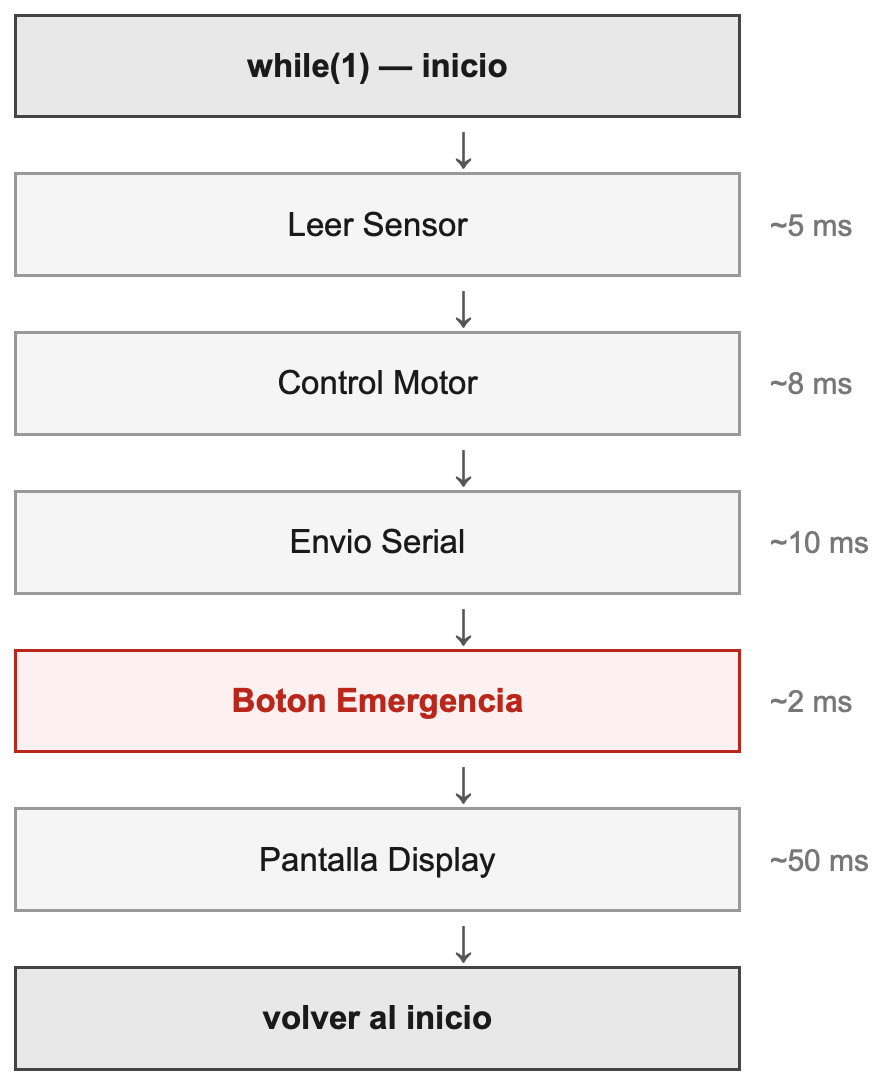
\includegraphics[width=0.9\linewidth]{images/problem_diagram.png}
    \caption{Diagrama del sistema secuencial con \texttt{while(1)} y tiempos acumulados por ciclo.}
    \label{fig:problem_diagram}
\end{figure}

\subsubsection{Discusión del caso}

En un entorno secuencial, todo el control reside en un bucle infinito donde el procesador ejecuta una instrucción tras otra. Para gestionar los tiempos, se suelen usar banderas o contadores de tiempo (como \texttt{millis()}). El código pregunta constantemente si es hora de leer el sensor o enviar datos, ejecutando las funciones solo cuando se cumple el tiempo establecido.

Sin embargo, el mayor riesgo de esto es el bloqueo por latencia. Si la tarea de "Actualizar pantalla" tarda 30 ms en completarse, el procesador quedará atrapado en esa función, impidiendo que el sensor se lea cada 10 ms. Esto genera una pérdida de datos y un control del motor errático. Además, el sistema se vuelve rígido, pues cualquier cambio en una tarea afecta el tiempo de todas las demás.

En esta tarea, la prioridad absoluta es el botón de emergencia, la cual es una medida de seguridad, por lo que no puede esperar a que un bucle termine su vuelta. Si el sistema está ocupado enviando un mensaje largo por el puerto serial y ocurre un accidente, un retraso de milisegundos en la detección del botón podría tener consecuencias catastróficas para el hardware o el operador \cite{verdugamonar_2025_controladores}.

Para asegurar el cumplimiento de los tiempos, es necesario transitar hacia una arquitectura orientada a eventos. Esto implica usar interrupciones para el botón de emergencia y los timers del sensor. Un RTOS facilitaría esto asignando prioridades, permitiendo que las tareas urgentes "expulsen" a las tareas lentas (como la pantalla) del CPU cuando sea necesario \cite{wirth_2022_superloop} \cite{verdugamonar_2025_controladores}.

\subsubsection{Solución propuesta}

La solución propuesta consiste en migrar de la arquitectura Super-loop a un RTOS (como FreeRTOS), donde cada tarea se ejecuta de forma independiente con su propio periodo y nivel de prioridad asignado por un Scheduler \cite{wirth_2022_superloop} \cite{verdugamonar_2025_controladores}. El botón de emergencia deja de ser una línea más dentro del bucle y se convierte en una interrupción hardware (ISR, del inglés, \textit{"Interrupt Service Routine"} o Rutina de Servicio de Interrupción), garantizando una respuesta en microsegundos sin importar qué esté haciendo el sistema \cite{wirth_2022_superloop}. El sensor se ejecuta como tarea periódica estricta cada 10 ms, el control del motor reacciona inmediatamente tras cada lectura, el envío serial corre cada 100 ms de forma independiente, y el display opera como tarea de fondo con la menor prioridad, de modo que sus 50 ms de ejecución nunca bloquean las tareas críticas. 

Así, el Scheduler se encarga de ceder y recuperar el CPU entre tareas según su urgencia, eliminando el problema central del Super-loop: que el tiempo de respuesta de cualquier evento dependa del tiempo de ciclo total del sistema.

\subsubsection{Respuesta Central: ¿Por qué no es suficiente un \texttt{while(1)}?}

Programar todo en un \texttt{while(1)} (conocido como arquitectura Super-loop) no es suficiente para sistemas complejos por tres razones críticas \cite{wirth_2022_superloop}.

En primer lugar, existe una falta de determinismo: el tiempo que tarda una vuelta completa del bucle depende de qué condiciones \texttt{if} se ejecutaron. Si la escritura en pantalla tarda 50\,ms, la lectura del sensor, que debe realizarse cada 10\,ms, se retrasará inevitablemente.

En segundo lugar, se produce una latencia inaceptable. Los eventos urgentes deben esperar a que el puntero del programa llegue a la línea donde se evalúa la condición correspondiente. En entornos de seguridad industrial, un retardo de 100\,ms puede ser suficiente para provocar un accidente.

Por último, se puede destacar que la arquitectura Super-loop es inescalable. A medida que se agregan funcionalidades, el código se vuelve frágil, por lo que modificar un simple \texttt{delay()} en una función puede comprometer el tiempo de respuesta de todo el sistema \cite{wirth_2022_superloop}.

En la Figura~\ref{fig:solution_diagram} se presenta el diagrama de la solución propuesta basada en un esquema con prioridades e interrupciones. El botón de emergencia se atiende mediante una interrupción hardware de máxima prioridad (ISR < 1 µs), garantizando respuesta inmediata. La lectura del sensor se ejecuta como tarea periódica cada 10 ms, seguida del control del motor como tarea reactiva. El envío serial se programa cada 100 ms, mientras que la actualización de la pantalla se ejecuta como tarea de fondo cuando el procesador está libre. Este enfoque asegura que las tareas críticas no sean bloqueadas por las de menor prioridad.

\begin{figure}[htbp]
    \centering
    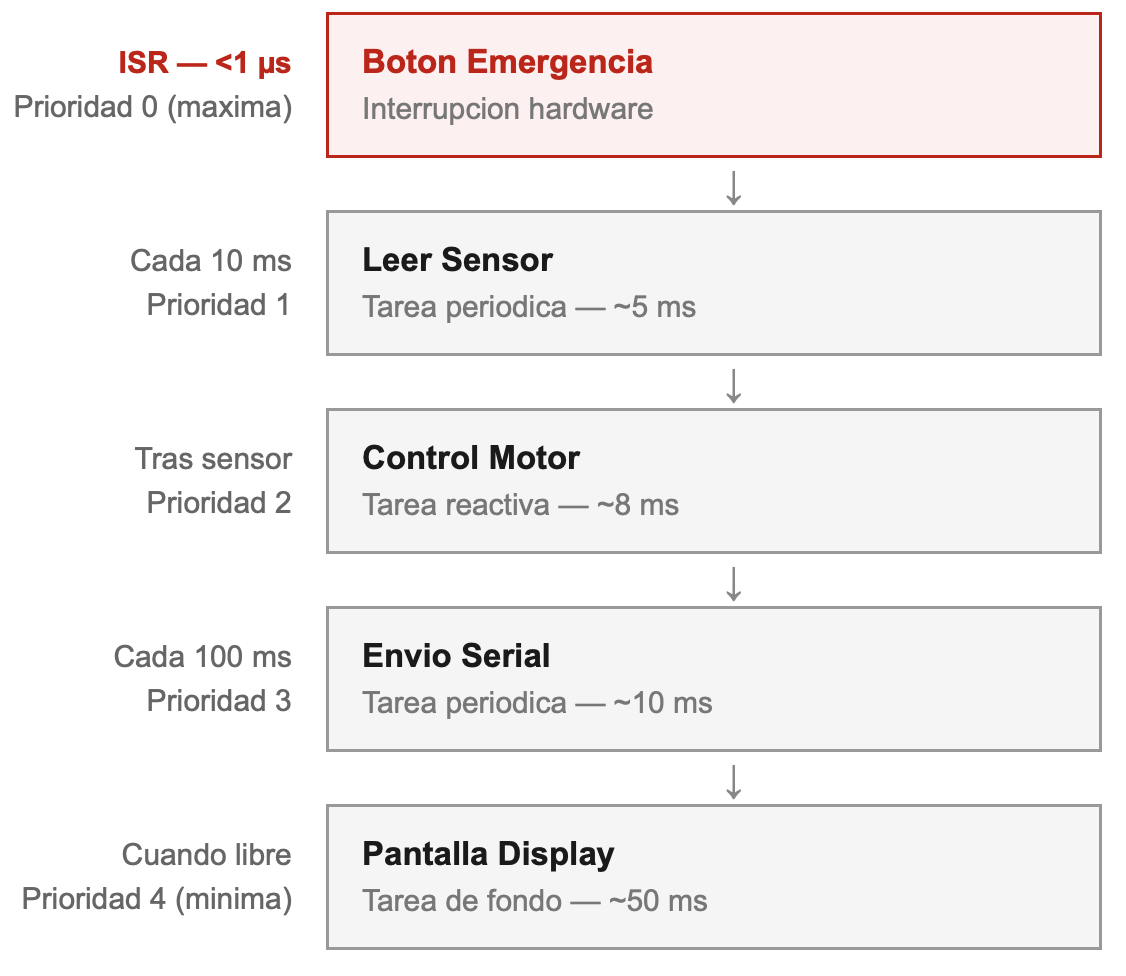
\includegraphics[width=0.9\linewidth]{images/solution_diagram.png}
    \caption{Arquitectura de solución basada en prioridades e interrupciones.}
    \label{fig:solution_diagram}
\end{figure}

\subsubsection{Material de consulta}

\paragraph{Interrupciones}

\begin{itemize}
    \item ¿Qué son?: Son mecanismos de hardware que permite al procesador suspender temporalmente la ejecución del programa principal para atender un evento urgente y específico \cite{sergio_2015_interrupciones}.
    
    \item ¿Cómo funcionan en un microcontrolador?: Actúa cuando ocurre un evento, el hardware completa la instrucción actual, guarda el estado del CPU en la pila (stack) y salta a una dirección de memoria fija llamada Vector de Interrupción, donde ejecuta la ISR (Rutina de Servicio de Interrupción). Al terminar, restaura el estado y vuelve al punto exacto donde se quedó \cite{sergio_2015_interrupciones}.
    
    \item ¿Qué problemas resuelven?: El Polling (preguntar constantemente). Sin interrupciones, el CPU pierde tiempo preguntando "¿ya presionaron el botón?" miles de veces por segundo \cite{sergio_2015_interrupciones}.

     \item ¿Qué riesgos implican?: Pueden causar corrupción de datos si no se manejan variables atómicas y, si son muy frecuentes, pueden provocar que el programa principal nunca se ejecute \cite{sergio_2015_interrupciones}.
     
\end{itemize}

\paragraph{Planificación y Scheduler}

\begin{itemize}
    \item ¿Qué es un scheduler?: Es el componente del núcleo (Kernel) encargado de decidir qué tarea (hilo) tiene el control del CPU en un momento dado \cite{ortega_2019_scheduler}.
    
    \item ¿Qué significa prioridad?: Es un valor numérico asignado a cada tarea. El Scheduler siempre favorecerá la ejecución de la tarea con mayor prioridad \cite{ortega_2019_scheduler}.
    
    \item ¿Qué es planificación preventiva y cooperativa?:
    
      \begin{itemize}

       \item Preventiva: El Scheduler puede "quitarle" el CPU a una tarea a la fuerza si aparece una de mayor prioridad. Es ideal para tiempo real.
       \item Cooperativa: Una tarea debe terminar o "ceder" voluntariamente el CPU para que otra pueda entrar. Si una tarea se queda en un bucle infinito, bloquea todo el sistema \cite{ortega_2019_scheduler}.
         
     \end{itemize}
  
\end{itemize}


\paragraph{Multitarea}

\begin{itemize}
    \item ¿Qué es concurrencia?: Es la capacidad del sistema para manejar múltiples tareas que parecen progresar simultáneamente, aunque en un solo núcleo se ejecuten una por una intercaladas \cite{sergio_2015_interrupciones} \cite{rivas_2012_multitarea}.
    
    \item Diferencia entre multitarea real y simulada:

       \begin{itemize}

       \item Real: Ocurre en procesadores de varios núcleos (Multi-core), donde cada núcleo ejecuta una tarea distinta físicamente al mismo tiempo.
       
       \item Simulada: Ocurre en microcontroladores de un solo núcleo mediante el Cambio de Contexto (Context Switching), alternando tareas tan rápido que el ojo humano no percibe la pausa \cite{rivas_2012_multitarea} \cite{verdugamonar_2025_controladores}.
         
       \end{itemize}
    
    \item Ejemplos en sistemas embebidos:

        \begin{itemize}

         \item Un sistema con RTOS como FreeRTOS donde:

             \begin{itemize}

             \item Una tarea maneja WiFi.
       
             \item Otra controla motores.

             \item Otra procesa datos de sensores \cite{verdugamonar_2025_controladores}.
         
            \end{itemize}
       
         \item En un ESP32 (doble núcleo):

               \begin{itemize}

               \item Núcleo 0 ejecuta la pila WiFi.
       
               \item Núcleo 1 ejecuta la lógica principal del usuario \cite{rivas_2012_multitarea}.
         
              \end{itemize}
         
        \end{itemize}
  
\end{itemize}

\paragraph{Sincronización}

\begin{itemize}
    \item ¿Qué es una condición de carrera?: Ocurre cuando dos o más tareas intentan modificar un recurso compartido (como una variable global) al mismo tiempo, dejando un resultado impredecible \cite{pez_2025_sincronizacion}.
    
    \item ¿Qué son semáforos y mutex?:

             \begin{itemize}

               \item Mutex: Abreviatura del inglés \textit{"mutual exclusion" }o exclusión mutua, es un "candado". Solo una tarea puede tener la llave para entrar a la sección crítica \cite{pez_2025_sincronizacion}.
       
               \item Semáforo: Es un "contador". Permite que un número limitado de tareas accedan a un recurso o sirve para señalizar entre tarea \cite{pez_2025_sincronizacion}.
              \end{itemize}

     \item ¿Qué es sección crítica?: Es la parte del código que accede a ese recurso compartido y que no debe ser interrumpida por ninguna otra tarea que use el mismo recurso \cite{sergio_2015_interrupciones} \cite{pez_2025_sincronizacion}.
     
\end{itemize}

% \begin{figure}[ht]          % Otra figura; [!b] sugiere colocación al pie de página
  % \centering
  % keepaspectratio asegura que no se deforme la relación de aspecto al escalar
  % width=0.9\linewidth establece el ancho relativo; se puede combinar con height=...
 %  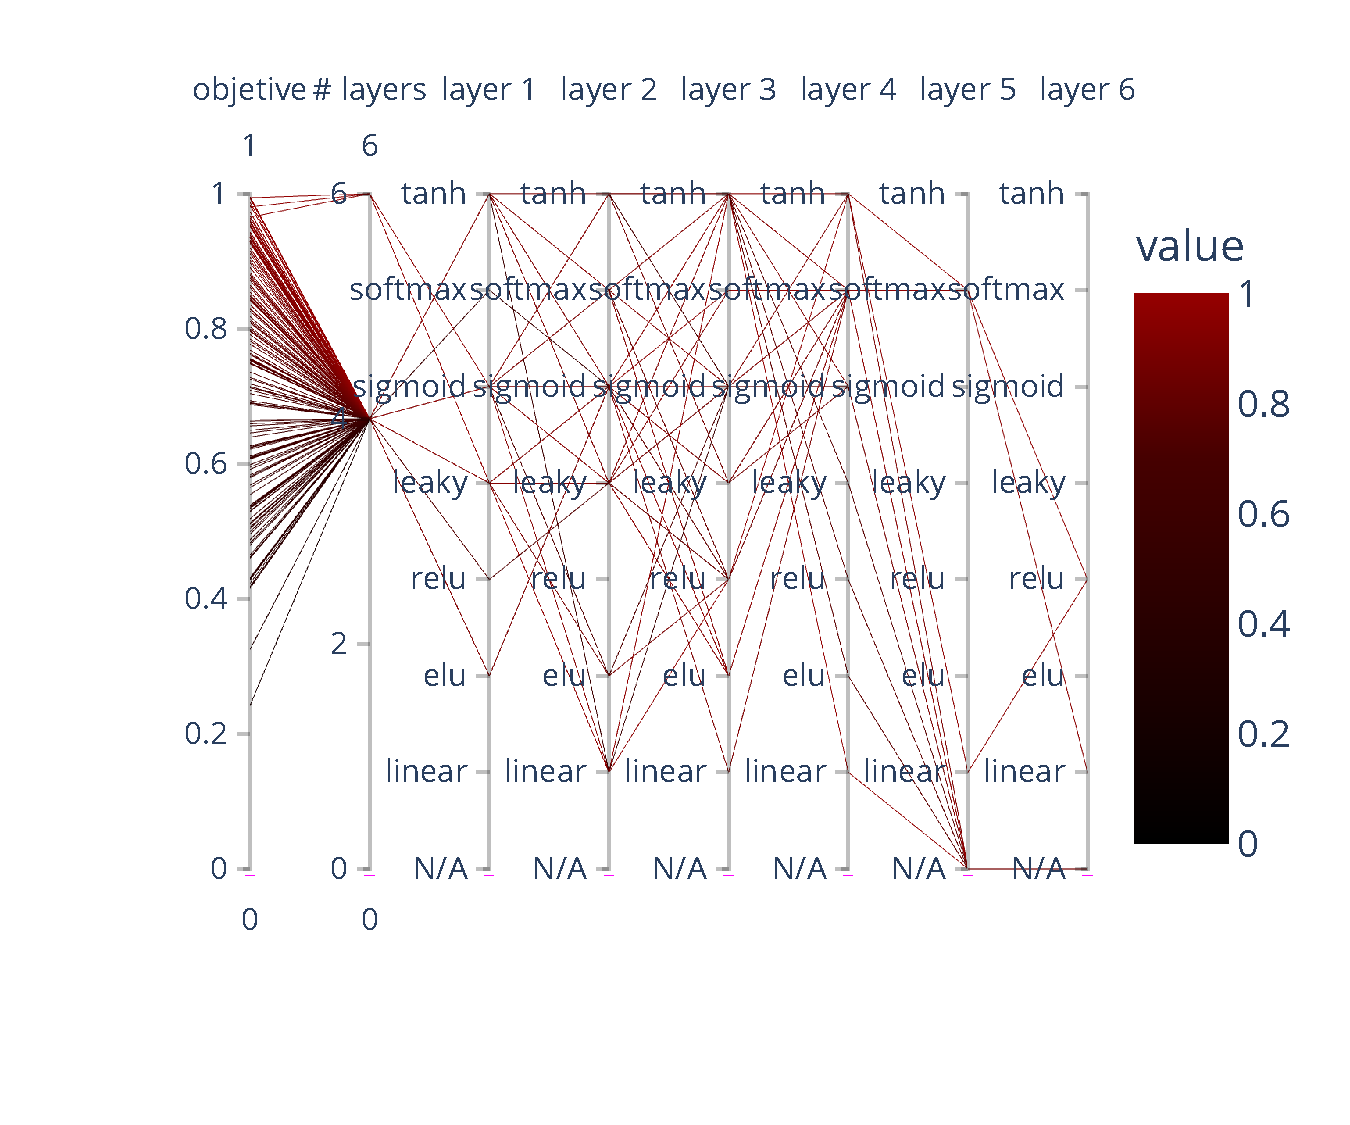
\includegraphics[keepaspectratio, width=0.9\linewidth]{images/act.pdf}
 %  \caption{Gráfico PGF de ejemplo (sustituible).}
  % \label{fig:ejemplo_pgf}   % Etiqueta para referencias cruzadas
%  \end{figure} 

% Fin de la sección de ejemplo.


\section{Desarrollo de talleres}\label{sec:talleres}
  % Esta sección describe equipo y procedimiento de manera simple.
% Reemplaza con tu propio contenido cuando enseñes o evalúes.

\subsection{Primer taller: Programación estructurada en sistemas embebidos} % Sub-sección metodológica

Este taller integrador se centra en el diseño y desarrollo de sistemas embebidos bajo el enfoque de la programación estructurada, integrando el modelado formal del sistema con su implementación práctica. A través de tres retos aplicados, el objetivo principal es desarrollar la capacidad de estructurar soluciones embebidas desde una perspectiva ingenieril, donde se debe justificar la selección del microcontrolador, organizar el código de forma modular y documentada, e implementar buenas prácticas en todo el desarrollo del mismo.

\subsubsection{RETO 1 – Sistema de Control de Acceso}\label{sec:reto1}
  

\begin{itemize}
    
    \item Análisis del problema:
    
     El sistema de control de acceso tiene como propósito verificar una contraseña digital ingresada mediante una combinación de botones físicos o un teclado matricial. Si la combinación es correcta, se activa una cerradura electrónica (servo motor o relé); en caso contrario, se contabilizan los intentos fallidos y, al superar el límite permitido, el sistema entra en un estado de bloqueo temporal.
     
        \begin{itemize}
             \item Identificación de Entradas y Salidas
                  \begin{itemize}       
                      \item Entradas del sistema:
                    
                            \begin{itemize}
                                 \item  Botones digitales (4 pulsadores) o teclado matricial 4x4 para ingreso de contraseña.

                                 \item Señal de reset (opcional): botón para reiniciar el sistema desde estado bloqueado.                      
                             \end{itemize}  
                             
                  \end{itemize}     

             \item Restricciones Técnicas
                     \begin{itemize}
                            \item Máximo 3 intentos fallidos antes de activar el bloqueo.
                            
                            \item Tiempo de bloqueo: 30 segundos.

                            \item La contraseña debe almacenarse en memoria no volátil (EEPROM) o en código.
                            
                            \item Temporización no bloqueante mediante millis()

                            \item El sistema debe retornar automáticamente al estado de espera tras el desbloqueo.
                     \end{itemize}
                     
             \item Variables Involucradas
                 
\begin{table}[h]
\centering
\caption{Variables del sistema de control de acceso}
\label{tab:Tabla_1_R1}
\footnotesize
\setlength{\tabcolsep}{4pt}
\renewcommand{\arraystretch}{1.5}
    
    \begin{tabularx}{\columnwidth}{|>{\raggedright\arraybackslash}p{3cm}|>{\centering\arraybackslash}p{1.5cm}|X|}
        \hline
        \textbf{Variable} & \textbf{Tipo} & \textbf{Descripción} \\
        
        \hline
        intentosFallidos & int & Contador de intentos incorrectos (0--3) \\ 
        
        \hline
        contrasenaIngresada & String & Secuencia de teclas presionadas por el usuario \\ 
        
        \hline
        contrasenaCorrecta & String & Contraseña almacenada en firmware \\ 
        
        \hline
        sistemaBloqueado & bool & Indica si el sistema está en estado de bloqueo \\ 
        
        \hline
        tiempoBloqueo & unsigned long & Marca de tiempo de inicio del bloqueo \\ 
        
        \hline
        accesoGarantizado & bool & Indicador de acceso concedido \\ \hline
\end{tabularx}
\end{table}
          
       \end{itemize}  
\end{itemize}


\begin{itemize}

       \item Flujograma del sistema
       
         A continuación se describe el algoritmo de comportamiento del sistema de control de acceso. El diagrama representa el flujo lógico completo desde el inicio hasta la resolución de cada evento de acceso.

             \begin{itemize}
             
                \item Descripción del Algoritmo (Pseudocódigo Estructurado):

                En el Algoritmo~\ref{alg:Algoritmo1} se puede observar el pseudocódigo, el cual, comienza declarando un bloque de INICIO que configura los periféricos. A continuación se evalúa si el sistema está bloqueado; en caso afirmativo, se verifica el temporizador y se libera al cumplirse 30 segundos. Si el sistema no está bloqueado, se espera la entrada del usuario. Cuando la contraseña está completa, se ejecuta la comparación: si es correcta, se activa el servo y el LED verde; si es incorrecta, se incrementa el contador de fallos y se evalúa si se alcanzó el límite. El proceso retorna al inicio del bucle en todos los casos.

                  
             \end{itemize}
             
\end{itemize}

\begin{algorithm}[h]
\caption{Algoritmo de Control de Acceso}
\label{alg:Algoritmo1}
\begin{algorithmic}[1]

\Statex \textbf{Inicialización:}
\State Inicializar pines, variables y servo en posición cerrada
\State $intentosFallidos = 0$
\State $sistemaBloqueado = false$

\While{true}

    \If{$sistemaBloqueado$}

        \If{$millis() - tiempoBloqueo \geq 30000$}
            \State $sistemaBloqueado = false$
            \State $intentosFallidos = 0$
            \State Apagar $LED\_ROJO$
        \EndIf

    \Else

        \State Leer tecla del teclado
        \State Agregar caracter a $contrasenaIngresada$

        \If{$|contrasenaIngresada| = |contrasenaCorrecta|$}

            \If{$contrasenaIngresada = contrasenaCorrecta$}

                \State Activar servo (abrir cerradura)
                \State Encender $LED\_VERDE$ durante 3 segundos
                \State Regresar servo a posicion cerrada
                \State $intentosFallidos = 0$

            \Else

                \State $intentosFallidos = intentosFallidos + 1$
                \State Hacer parpadear $LED\_ROJO$

                \If{$intentosFallidos \geq 3$}
                    \State $sistemaBloqueado = true$
                    \State $tiempoBloqueo = millis()$
                \EndIf

            \EndIf

            \State $contrasenaIngresada = " "$

        \EndIf

    \EndIf

\EndWhile

\end{algorithmic}
\end{algorithm} 
%\bigskip


\begin{itemize}

    \item Justificación técnica del microcontrolador seleccionado

        \begin{itemize}

             \item Microcontrolador Seleccionado: Arduino UNO (ATmega328P): El Arduino UNO con microcontrolador ATmega328P resulta adecuado para este sistema debido a su disponibilidad, bajo costo, amplia comunidad de soporte y suficiente cantidad de pines para los periféricos requeridos\cite{Arduino_datasheet}.

             \item Análisis de Pines Requeridos:
              El ATmega328P dispone de 14 pines digitales (6 con PWM) y 6 analógicos, cubriendo ampliamente los 12 pines requeridos con margen de expansión.
              
                 

\begin{table}[h]
\caption{Análisis de Pines Requeridos}
\label{tab:Tabla_2_R1}
\centering
\renewcommand{\arraystretch}{1.2}
\begin{tabular}{p{2.5cm} p{3.5cm} p{2cm}}
\toprule
\textbf{Componente} & \textbf{Pines Requeridos} & \textbf{Tipo} \\
\midrule
Teclado matricial 4x4 & 8 pines digitales (4 filas + 4 columnas) & Digital I/O \\
LED verde & 1 pin digital & Digital OUTPUT \\
LED rojo & 1 pin digital & Digital OUTPUT \\
Servo motor & 1 pin PWM & PWM OUTPUT \\
Buzzer & 1 pin digital & Digital OUTPUT \\
\midrule
\textbf{Total} & \textbf{12 pines} & --- \\
\bottomrule
\end{tabular}
\end{table}

             \item Capacidad de Procesamiento

                 \begin{itemize}
                 
                       \item CPU: ATmega328P @ 16 MHz
                       \item Memoria Flash: 32 KB (programa ocupa < 5 KB)
                       \item SRAM: 2 KB (suficiente para buffers de contraseña y variables de estado)
                       \item EEPROM: 1 KB (almacenamiento persistente de contraseña) 
                       
                 \end{itemize}

             \item Consumo Energético

                  \begin{itemize}
                 
                       \item Consumo activo: ~46 mA @ 5V = ~230 mW
                       \item LED: ~20 mA c/u con resistencia limitadora de 220 ohms
                       \item Servo SG90: ~100–250 mA en movimiento
                       \item Alimentación recomendada: 5V/1A (USB o adaptador)
                       
                 \end{itemize}
                 
             \item Componentes Auxiliares
                  \begin{table}[h]
\caption{Componentes Electrónicos del Sistema}
\label{tab:Tabla_3_R1}
\centering

\footnotesize
\setlength{\tabcolsep}{4pt}
\renewcommand{\arraystretch}{1.5}

\begin{tabularx}{\columnwidth}{|>{\raggedright\arraybackslash}p{3cm}|>{\centering\arraybackslash}p{1.5cm}|X|}
\hline
\textbf{Componente} & \textbf{Cant.} & \textbf{Especificación / Función} \\
\hline
LED verde 5mm & 1 & 3.3V, 20mA. Indicador de acceso correcto. \\
\hline
LED rojo 5mm & 1 & 3.3V, 20mA. Indicador de error o bloqueo. \\
\hline
Resistencia 220 $\Omega$ & 2 & 1/4 W. Limitación de corriente para los LEDs. \\
\hline
Buzzer pasivo & 1 & 5V. Generación de señal sonora de retroalimentación. \\
\hline
Protoboard / PCB & 1 & 830 puntos. Montaje físico del circuito. \\
\hline
\end{tabularx}

\end{table}

             \item Esquema de Conexión

             En la Figura \ref{fig:Imagen_1_R1} se observa el diagrama de conexión correspondiente al funcionamiento de este circuito, desarrollado a través del programa de circuitado. A continuación se mencionan las conexiones establecidas en el proyecto:
             \begin{itemize}
                 \item Teclado 4x4: Filas a pines D4, D5, D6, D7 — Columnas a pines D8, D9, D10, D11
                \item LED verde: Pin D12 → Resistencia 220 ohms → Ánodo LED → Cátodo → GND
                \item LED rojo: Pin D13 → Resistencia 220 ohms → Ánodo LED → Cátodo → GND
                \item Servo SG90: Cable señal a Pin D3 (PWM), VCC a 5V, GND a GND
                \item Buzzer: Pin D2 → Buzzer (+) → GND
                \item Alimentación: 5V desde USB o regulador 7805

             \end{itemize}
             \textit{EasyEDA}.
                  \begin{figure}[h]
                  \centering
                  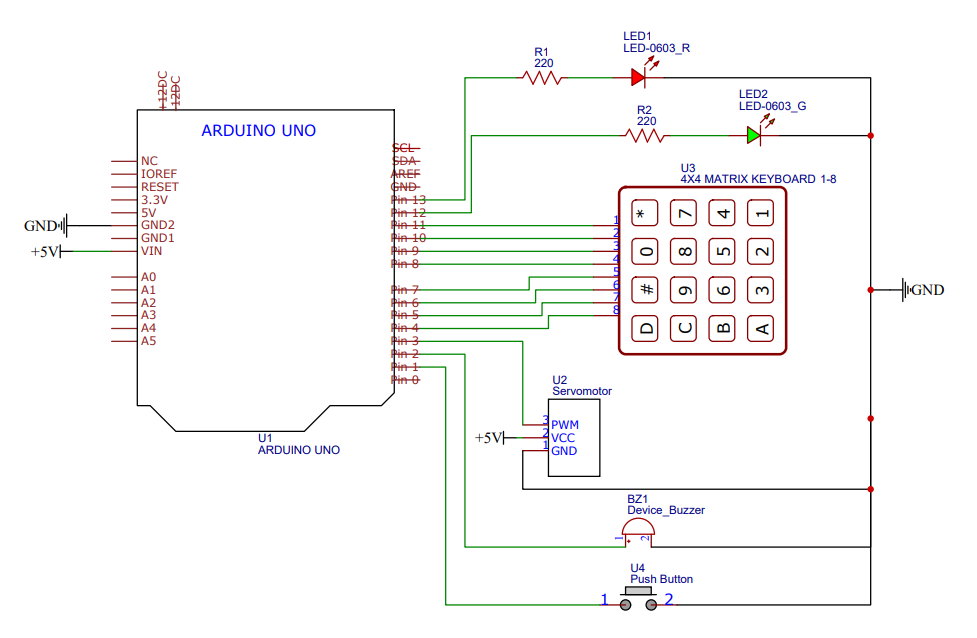
\includegraphics[width=\columnwidth]{images/Imagen_1R1.png}
                  \caption{Esquemático de Conexión Reto 1}
                  \label{fig:Imagen_1_R1}
                  \end{figure}
             
        \end{itemize}
  
\end{itemize}

\begin{itemize}
      \item Código documentado
      
      El código está organizado de forma modular separando la inicialización de hardware, la lógica de verificación, el control de la cerradura y la gestión de estados de bloqueo. Se evita el uso de delay() para garantizar temporización no bloqueante.

      \begin{lstlisting}[caption={Implementación de Control de Acceso con Teclado y Servo}, label={lst:control-acceso}]
#include <Keypad.h>
#include <Servo.h>

// --- Definicion de pines ---
#define PIN_SERVO       3
#define PIN_BUZZER      2
#define PIN_LED_VERDE   12
#define PIN_LED_ROJO    13
#define PIN_BOTON       A0

// --- Configuracion del teclado 4x4 ---
const byte FILAS    = 4;
const byte COLUMNAS = 4;

char teclas[FILAS][COLUMNAS] = {
  { '1', '2', '3', 'A' },
  { '4', '5', '6', 'B' },
  { '7', '8', '9', 'C' },
  { '*', '0', '#', 'D' }
};

byte pinesFilas[FILAS] =
  { 11, 10, 9, 8 };
byte pinesColumnas[COLUMNAS] =
  {  7,  6, 5, 4 };

Keypad teclado =
  Keypad(makeKeymap(teclas),
         pinesFilas,
         pinesColumnas,
         FILAS,
         COLUMNAS);

// --- Servo ---
Servo servo;
#define ANGULO_ABIERTO  90
#define ANGULO_CERRADO   0

// --- Variables de control de 
acceso ---
const String PASSWORD = "1234";
const byte MAX_INTENTOS = 3;
const unsigned long TIEMPO_BLOQUEO
= 30000;

// --- Estado general ---
String entradaActual = "";
byte intentosFallidos = 0;
bool bloqueado = false;
unsigned long tiempoBloqueo = 0;

// --- Servo temporizado ---
bool puertaAbierta = false;
unsigned long tiempoServo = 0;

// --- Buzzer no bloqueante ---
bool buzzerActivo = false;
unsigned long tiempoBeep = 0;
int duracionBeep = 0;

// --- Parpadeo LED rojo ---
unsigned long tiempoBlink = 0;
bool estadoBlink = false;
byte parpadeosPendientes = 0;
bool ledRojoFijo = false;

// --- Anti-rebote boton ---
unsigned long ultimoDebounce = 0;
const unsigned long 
DEBOUNCE_DELAY = 50;

// ===================
void inicializarHardware() {
  pinMode(PIN_LED_VERDE, OUTPUT);
  pinMode(PIN_LED_ROJO, OUTPUT);
  pinMode(PIN_BUZZER, OUTPUT);
  pinMode(PIN_BOTON, 
  INPUT_PULLUP);
  servo.attach(PIN_SERVO);
  servo.write(ANGULO_CERRADO);
  digitalWrite(PIN_LED_VERDE, LOW);
  digitalWrite(PIN_LED_ROJO,  LOW);
  Serial.println("Sistema de
  acceso listo");
}

// ===================
void beep(int frecuencia,
          int duracion) {
  tone(PIN_BUZZER, frecuencia);
  buzzerActivo = true;
  tiempoBeep   = millis();
  duracionBeep = duracion;
}

// ===================
void actualizarBuzzer() {
  if (buzzerActivo) {
    if (millis() - tiempoBeep
        >= duracionBeep) {
      noTone(PIN_BUZZER);
      buzzerActivo = false;
    }
  }
}

// ===================
void actualizarServo() {
  if (puertaAbierta) {
    if (millis() - tiempoServo
        >= 3000) {
      servo.write(ANGULO_CERRADO);
      digitalWrite(PIN_LED_VERDE,
      LOW);
      puertaAbierta = false;
    }
  }
}

// ===================
void actualizarBlink() {
  if (!estadoBlink) return;
  if (millis() - tiempoBlink < 300)
    return;
  tiempoBlink = millis();
  bool ledActual =
    digitalRead(PIN_LED_ROJO);
  if (!ledActual) {
    digitalWrite(PIN_LED_ROJO, HIGH);
    parpadeosPendientes--;
  } else {
    if (parpadeosPendientes == 0) {
      estadoBlink = false;
      digitalWrite(PIN_LED_ROJO,
        ledRojoFijo ? HIGH : LOW);
    } else {
      digitalWrite(PIN_LED_ROJO, LOW);
    }
  }
}

// ===================
void accesoAprobado() {
  intentosFallidos  = 0;
  estadoBlink       = false;
  ledRojoFijo       = false;
  digitalWrite(PIN_LED_ROJO,  LOW);
  digitalWrite(PIN_LED_VERDE, HIGH);
  servo.write(ANGULO_ABIERTO);
  puertaAbierta = true;
  tiempoServo   = millis();
  beep(2000, 150);
}

// ===================
void accesoNegado() {
  intentosFallidos++;
  if (intentosFallidos < 
  MAX_INTENTOS)
  {
    parpadeosPendientes = 2;
    ledRojoFijo         = false;
  } else {
    parpadeosPendientes = 3;
    ledRojoFijo         = true;
  }
  estadoBlink = true;
  tiempoBlink = millis();
  digitalWrite(PIN_LED_ROJO, LOW);
  beep(500, 500);
  if (intentosFallidos >= 
  MAX_INTENTOS)
  {
    bloqueado     = true;
    tiempoBloqueo = millis();
  }
}

// ===================
void verificarPassword() {
  if (entradaActual == PASSWORD)
    accesoAprobado();
  else
    accesoNegado();
  entradaActual = "";
}

// ===================
void procesarTecla(char tecla) {
  if (tecla == '#') {
    verificarPassword();
    return;
  }
  if (tecla == '*') {
    entradaActual = "";
    beep(1000, 100);
    return;
  }
  entradaActual += tecla;
  if (entradaActual.length()
      > PASSWORD.length()) {
    entradaActual = "";
    beep(500, 200);
  }
}

// ===================
void leerBoton() {
  if (digitalRead(PIN_BOTON) == LOW) {
    if (millis() - ultimoDebounce
        > DEBOUNCE_DELAY) {
      bloqueado        = false;
      intentosFallidos = 0;
      entradaActual    = "";
      estadoBlink      = false;
      ledRojoFijo      = false;
      digitalWrite(PIN_LED_ROJO, LOW);
      digitalWrite(PIN_LED_VERDE, 
      LOW);
      beep(1800, 200);
      ultimoDebounce = millis();
    }
  }
}

// ===================
void setup() {
  Serial.begin(9600);
  inicializarHardware();
}

// ===================
void loop() {
  actualizarBuzzer();
  actualizarServo();
  actualizarBlink();
  leerBoton();
  if (bloqueado) {
    if (millis() - tiempoBloqueo
        >= TIEMPO_BLOQUEO) {
      bloqueado        = false;
      intentosFallidos = 0;
      estadoBlink      = false;
      ledRojoFijo      = false;
      digitalWrite(PIN_LED_ROJO, LOW);
      beep(1500, 300);
    }
    return;
  }
  char tecla = teclado.getKey();
  if (tecla) procesarTecla(tecla);
}
\end{lstlisting}
      
\end{itemize}




\subsubsection{RETO 2 – Sistema de Control de Acceso}\label{sec:reto2}
  \begin{itemize}
    \item Análisis del problema
        \begin{itemize}
        
            \item Descripción general:
            El sistema de monitoreo con alarmas supervisa continuamente una variable física y clasifica su valor en tres niveles operativos: Normal, Advertencia y Crítico. Para cada nivel se activan indicadores visuales y/o sonoros diferenciados. Se implementa histéresis para evitar oscilaciones inestables en los umbrales de transición.

        \end{itemize} 

    \item Identificación de Entradas y Salidas
        \begin{itemize}
            
            \item Entradas:
                \begin{itemize}
                    \item  Sensor de temperatura (señal analógica o digital).

                    \item Botón de silencio de alarma (opcional).                   
                \end{itemize}
            
            \item Salidas:
                \begin{itemize}
                    \item  LED verde: estado Normal.
                    
                    \item LED amarillo: estado Advertencia.    
                    \item LED rojo: estado Crítico. 

                    \item Buzzer: alarma sonora en Advertencia y Crítico.
                    
                \end{itemize}

    \item Restricciones técnicas
        \begin{itemize}
            \item Los umbrales deben ser configurables mediante constantes.

            \item Implementación obligatoria de histéresis para evitar inestabilidad en los límites.
            
            \item El sistema debe funcionar en ciclo continuo con temporización no bloqueante.
            
            \item La lectura del sensor debe ser promediada para reducir ruido.
            
        \end{itemize}
       
    \item Definición de umbrales y variables:

    En la Tabla~\ref{tab:Tabla_1_R2}, se observa la definición de las variables con sus respectivas descripciones y justificación. Reconocer las variables a utilizar sera de ayuda a la hora de realizar el código.

    

\begin{table}[!ht]
\centering
\caption{Definición de Umbrales y Variables}
\label{tab:Tabla_1_R2}
\footnotesize
\setlength{\tabcolsep}{3pt}
\renewcommand{\arraystretch}{1.3}
    \begin{tabularx}{\columnwidth}{|p{3.2cm}|p{2cm}|X|}

        \hline
        \textbf{Variable} & \textbf{Valor} & \textbf{Descripción} \\ 

        \hline UMBRAL\_ADVERTENCIA & const = 30°C & Umbral para activar advertencia \\ 

        \hline UMBRAL\_CRITICO & const = 40°C & Umbral para nivel crítico \\ 

        \hline HISTERESIS & const = 2°C & Margen para evitar fluctuaciones \\ 

        \hline temperaturaActual & float & Valor del sensor en °C \\ 

        \hline estadoActual & enum & NORMAL, ADVERTENCIA, CRÍTICO \\ 
    
        \hline tiempoUltimaLectura & unsigned long & Timestamp de la lectura \\ 
        
        \hline
    \end{tabularx}
\end{table}

    \item Flujograma del Sistema

    El algoritmo, que se observa como Algoritmo ~\ref{alg:control_temp},
    funciona en ciclo continuo, e implementa un sistema de monitoreo de temperatura basado en una máquina de estados con tres niveles: NORMAL, ADVERTENCIA y CRÍTICO. Cada 500 ms se realiza una nueva lectura del sensor, se calcula la temperatura y se determina el estado del sistema aplicando histéresis. En función del estado, se activan los indicadores correspondientes.
    
    

\begin{algorithm}[t]
\caption{Control de Temperatura con Histéresis}
\label{alg:control_temp}
\begin{algorithmic}[1]

\Statex \textbf{INICIO}
\State Inicializar pines, LCD, sensor
\State $\text{estadoActual} \gets \text{NORMAL}$

\Loop \ \textbf{PRINCIPAL} (cada 500 ms)
    \State $\text{temperaturaActual} \gets \text{leerSensor}()$
    
    \If{$\text{estadoActual} = \text{NORMAL}$}
        \If{$\text{temperaturaActual} \geq \text{UMBRAL\_ADVERTENCIA}$}
            \State $\text{estadoActual} \gets \text{ADVERTENCIA}$
        \EndIf

    \ElsIf{$\text{estadoActual} = \text{ADVERTENCIA}$}
        \If{$\text{temperaturaActual} \geq \text{UMBRAL\_CRITICO}$}
            \State $\text{estadoActual} \gets \text{CRITICO}$
        \ElsIf{$\text{temperaturaActual} < (\text{UMBRAL\_ADVERTENCIA} - \text{HISTERESIS})$}
            \State $\text{estadoActual} \gets \text{NORMAL}$
        \EndIf

    \ElsIf{$\text{estadoActual} = \text{CRITICO}$}
        \If{$\text{temperaturaActual} < (\text{UMBRAL\_CRITICO} - \text{HISTERESIS})$}
            \State $\text{estadoActual} \gets \text{ADVERTENCIA}$
        \EndIf
    \EndIf

    \State actualizarIndicadores($\text{estadoActual}$)
    \State mostrarEnLCD($\text{temperaturaActual, estadoActual}$)
\EndLoop
\Statex \textbf{FIN}

\end{algorithmic}
\end{algorithm}

    \item Justificación técnica del microcontrolador
        \begin{itemize}
            \item Microcontrolador Seleccionado: Arduino UNO (ATmega328P)

            El mismo microcontrolador del reto anterior es suficiente para este segundo reto.  Para usar el DHT21, se requiere únicamente un pin digital con protocolo one-wire.

            \item Análisis de Pines Requeridos:

            En la Tabla~\ref{tab:Tabla_2_R2}, se observan los pines solicitados para el correcto funcionamiento del programa.

            
\begin{table}[ht]
\caption{Análisis de Pines Requeridos (Sistema de Monitoreo)}
\label{tab:Tabla_2_R2}
\centering
\renewcommand{\arraystretch}{1.3}
\begin{tabularx}{\columnwidth}{X p{2.0cm} p{2.0cm}}
\toprule
\textbf{Componente} & \textbf{Pin} & \textbf{Tipo} \\
\midrule
Sensor NTC / DHT21 & A0 o D2 & Analógico / Digital \\
LED verde & D9 & Digital OUTPUT \\
LED amarillo & D10 & Digital OUTPUT \\
LED rojo & D11 & Digital OUTPUT \\
Buzzer & D8 & Digital OUTPUT \\

\midrule
\textbf{Total} & \textbf{6 pines} & --- \\
\bottomrule
\end{tabularx}
\end{table}

            \item Componentes auxiliares

            El sistema emplea como elemento principal de medición un sensor de temperatura DHT21. La visualización de la información se realiza mediante monitor serial en el Arduino IDE, lo que optimiza el uso de pines del microcontrolador.
            
            Para la señalización del estado del sistema se utilizan tres LEDs de 5 mm (verde, amarillo y rojo) de 20 mA, cada uno con su respectiva resistencia limitadora de 220 ohms para protección. Además, se integra un buzzer activo de 5 V y aproximadamente 85 dB que funciona como alarma sonora en condiciones críticas, reforzando la advertencia al usuario.

            \item Esquema de conexión 

            En la Figura \ref{fig:Imagen_1R2} se observa el diagrama de conexión correspondiente al funcionamiento de este circuito, desarrollado a través del programa de circuitado. A continuación se mencionan las conexiones realizadas:
            \begin{itemize}
                \item Sensor DHT21: D2 → pin DATA (resistencia pull-up 10k ohms entre DATA y VCC), VCC a 5V, GND a GND
                \item LED verde: D9 → 220 ohms → LED → GND
                \item LED amarillo: D10 → 220 ohms → LED → GND
                \item LED rojo: D11 → 220 ohms → LED → GND
                \item Buzzer: D8 → buzzer (+) → GND
            \end{itemize}
            \textit{EasyEDA}.
                  \begin{figure}[h]
                  \centering
                  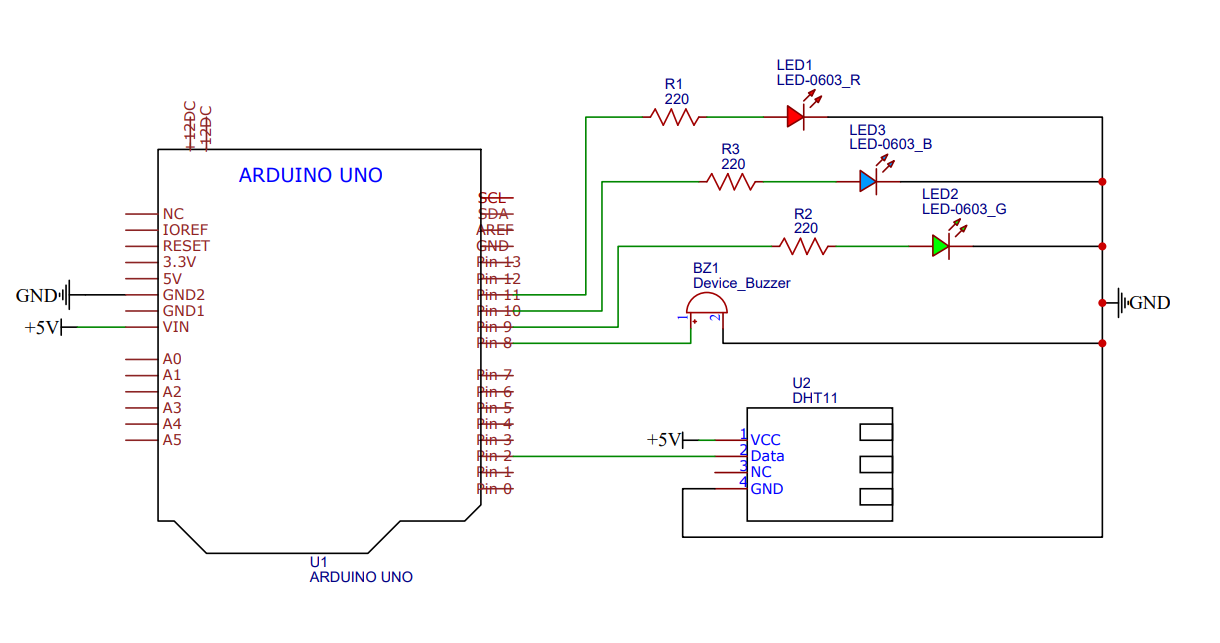
\includegraphics[width=\columnwidth]{images/Imagen_1R2.png}
                  \caption{Esquemático de Conexión Reto 2}
                  \label{fig:Imagen_1R2}
                  \end{figure}
            
        \end{itemize}

    \item Código Documentado

    El código propuesto documentado se encuentra registrado a continuación:
    \begin{lstlisting}[caption={Sistema de Monitoreo de Temperatura con DHT11}, label={lst:monitoreo-temperatura}]
#include <DHT.h>

// --- Pines ---
const int PIN_SENSOR       = 2;
const int PIN_LED_VERDE    = 9;
const int PIN_LED_AMARILLO = 10;
const int PIN_LED_ROJO     = 11;
const int PIN_BUZZER       = 8;

// --- Configuracion DHT11 ---
#define DHTTYPE DHT11
DHT dht(PIN_SENSOR, DHTTYPE);

// --- Umbrales de temperatura ---
const float UMBRAL_ADVERTENCIA = 30.0;  
const float UMBRAL_CRITICO     = 40.0;  
const float HISTERESIS         = 2.0;   

// --- Enumeracion de estados ---
enum EstadoSistema 
{ NORMAL, ADVERTENCIA, CRITICO };
EstadoSistema estadoActual = NORMAL;

// --- Variables de temporizacion ---
unsigned long tiempoUltimaLectura = 0;
const long    INTERVALO_LECTURA   = 2000;
unsigned long tiempoBuzzer        = 0;
bool          estadoBuzzer        = false;

float leerTemperatura() {
  float temp = dht.readTemperature();
  if (isnan(temp)) {
    Serial.println("Error al leer 
    el DHT11");
    return -999.0;
  }
  return temp;
}

void evaluarEstado(float temperatura) {
  if (temperatura == -999.0) return;
  switch (estadoActual) {
    case NORMAL:
      if (temperatura >= 
      UMBRAL_ADVERTENCIA)
        estadoActual = ADVERTENCIA;
      break;
    case ADVERTENCIA:
      if (temperatura >= UMBRAL_CRITICO)
        estadoActual = CRITICO;
      else if (temperatura < 
               UMBRAL_ADVERTENCIA 
               - HISTERESIS)
        estadoActual = NORMAL;
      break;
    case CRITICO:
      if (temperatura < UMBRAL_CRITICO 
      - HISTERESIS)
        estadoActual = ADVERTENCIA;
      break;
  }
}

void actualizarLEDs() {
  digitalWrite(PIN_LED_VERDE,
               estadoActual == NORMAL);
  digitalWrite(PIN_LED_AMARILLO,
               estadoActual == 
               ADVERTENCIA);
  digitalWrite(PIN_LED_ROJO,
               estadoActual == 
               CRITICO);
}

void gestionarBuzzer() {
  if (estadoActual == NORMAL) {
    noTone(PIN_BUZZER);
    return;
  }
  long intervalo = 
    (estadoActual == ADVERTENCIA)
    ? 1000 : 250;
  if ((millis() - tiempoBuzzer)
  >= intervalo) {
    tiempoBuzzer = millis();
    estadoBuzzer = !estadoBuzzer;
    if (estadoBuzzer)
      tone(PIN_BUZZER, 1500,
      intervalo / 2);
    else
      noTone(PIN_BUZZER);
  }
}

void setup() {
  Serial.begin(9600);
  dht.begin();
  pinMode(PIN_LED_VERDE,    OUTPUT);
  pinMode(PIN_LED_AMARILLO, OUTPUT);
  pinMode(PIN_LED_ROJO,     OUTPUT);
  pinMode(PIN_BUZZER,       OUTPUT);
  Serial.println("Sistema de 
  Monitoreo - Activo");
}

void loop() {
  unsigned long ahora = millis();
  if (ahora - tiempoUltimaLectura >= 
      INTERVALO_LECTURA) {
    tiempoUltimaLectura = ahora;
    float temperatura = leerTemperatura();
    evaluarEstado(temperatura);
    actualizarLEDs();
    Serial.print("T=");
    Serial.print(temperatura);
    Serial.print(" Estado=");
    Serial.println(estadoActual);
  }
  gestionarBuzzer();
}
\end{lstlisting}


    
    \end{itemize}  
\end{itemize}


\subsubsection{RETO 3 – Sistema de Control de Acceso}\label{sec:reto3}
  \begin{itemize}
    \item Análisis del problema
        \begin{itemize}
        
            \item Descripción general:
            El sistema de riego automático para cultivo de tomate monitorea continuamente la humedad relativa del ambiente mediante un sensor digital DHT11. Cuando la humedad desciende por debajo de un umbral mínimo, activa una bomba de agua (mediante relé) para iniciar el riego. El proceso se detiene al alcanzar el nivel de humedad óptimo. Se implementa histéresis para evitar ciclos de encendido/apagado rápidos y temporización no bloqueante para garantizar un funcionamiento secuencial estable. La información del sistema se visualiza en una pantalla OLED I2C de 0.96".

        \end{itemize} 

        \item Identificación de Entradas y Salidas
        \begin{itemize}
            
            \item Entradas:
                \begin{itemize}
                    \item  Sensor DHT11: señal digital en pin D2 (humedad relativa y temperatura).

                    \item Botón de riego manual (override): pin digital D3.                  
                \end{itemize}
            
            \item Salidas:
                \begin{itemize}
                    \item Módulo relé 5V: activa/desactiva la bomba de agua.
                    \item LED verde: humedad adecuada (IDLE).    
                    \item LED azul/amarillo: riego activo (REGANDO).
                    \item LED rojo: humedad crítica baja (ALARMA).
                    \item Pantalla OLED I2C 0.96" 128x64: visualización del porcentaje de humedad y estado del sistema.
                \end{itemize}
        \end{itemize}

        \item Restricciones técnicas
            \begin{itemize}
                \item No se debe usar delay() en el ciclo principal.
                \item Implementación de histéresis en umbrales de humedad.
                \item El sistema debe operar de forma completamente autónoma sin intervención humana.
                \item Separación de la lógica de negocio del control de hardware.
                \item El DHT11 requiere un intervalo mínimo de 2000 ms entre lecturas.
                \item Tiempo mínimo de riego: 5 segundos para evitar micro-ciclos.
                
            \end{itemize}

        \item Definición de umbrales y variables:

        En la Tabla~\ref{tab:Table_1_R3}, se observa la definición de las variables con sus respectivas descripciones y justificación. Reconocer las variables a utilizar sera de ayuda a la hora de realizar el código.

        \begin{table}[ht]
\caption{Variables Involucradas (Sistema de Riego Automático)}
\label{tab:Table_1_R3}
\centering
\renewcommand{\arraystretch}{1.3}
\begin{tabularx}{\columnwidth}{X p{2.0cm} p{2.0cm}}
\toprule
\textbf{Variable} & \textbf{Tipo} & \textbf{Valor / Rango} \\
\midrule
UMBRAL\_SECO   & const int    & 30\%       \\
UMBRAL\_HUMEDO & const int    & 70\%       \\
UMBRAL\_ALARMA & const int    & 20\%       \\
HISTERESIS     & const int    & 5\%        \\
humedadActual  & float        & 0--100\%   \\
estadoRiego    & enum         & IDLE / REGANDO / ALARMA \\
bombaActiva    & bool         & true / false \\
tiempoInicioRiego & unsigned long & ms      \\
tiempoMinRiego & const long   & 5000 ms    \\
\midrule
\textbf{Total} & \textbf{9 variables} & --- \\
\bottomrule
\end{tabularx}
\end{table}

        \item Flujograma del Sistema

        El sistema opera mediante un ciclo continuo con lecturas periódicas del sensor DHT11 cada 2000 ms. La lógica de control de la bomba se ejecuta basándose en el estado actual y los valores de humedad medidos, aplicando histéresis para garantizar estabilidad.

        \begin{algorithm}[ht]
\caption{Algoritmo de Sistema de Riego Automático}
\label{alg:Algoritmo_Riego}
\begin{algorithmic}[1]
\Statex \textbf{Inicialización:}
\State Inicializar pines, YI69, relé en OFF y pantalla OLED
\State $estadoRiego = IDLE$
\State $bombaActiva = false$
\While{true}
    \If{$millis() - tiempoUltimaLectura \geq 2000$}
        \State $tiempoUltimaLectura = millis()$
        \State $humedadActual = dht.readHumidity()$
        \If{$humedadActual = invalida$}
            \State Mostrar error en OLED
        \Else
            \If{$estadoRiego = IDLE$}
                \If{$humedadActual < UMBRAL\_ALARMA$}
                    \State $estadoRiego = ALARMA$
                    \State $activarBomba()$
                \ElsIf{$humedadActual \leq UMBRAL\_SECO$}
                    \State $estadoRiego = REGANDO$
                    \State $activarBomba()$
                    \State $tiempoInicioRiego = millis()$
                \EndIf
            \ElsIf{$estadoRiego = REGANDO$}
                \If{$millis() - tiempoInicioRiego \geq tiempoMinRiego$}
                    \If{$humedadActual \geq UMBRAL\_HUMEDO$}
                        \State $estadoRiego = IDLE$
                        \State $desactivarBomba()$
                    \EndIf
                \EndIf
            \ElsIf{$estadoRiego = ALARMA$}
                \State $activarBomba()$
                \If{$humedadActual \geq (UMBRAL\_SECO + HISTERESIS)$}
                    \State $estadoRiego = IDLE$
                    \State $desactivarBomba()$
                \EndIf
            \EndIf
            \State $actualizarIndicadores(estadoRiego)$
            \State $mostrarP(humedadActual,\ estadoRiego)$
        \EndIf
    \EndIf
    \State $gestionarBuzzerAlarma()$
    \State $verificarBotonManual()$
\EndWhile
\end{algorithmic}
\end{algorithm}

        \item Justificación técnica del microcontrolador
            \begin{itemize}
                \item Microcontrolador Seleccionado: Arduino UNO (ATmega328P)
    
                Para el sistema de riego autónomo se selecciona el Arduino UNO. El ATmega328P es suficiente para este prototipo educativo dado que el DHT11 utiliza un único pin digital y la pantalla OLED SSD1306 se comunica por I2C, ocupando únicamente los pines A4 y A5. Para aplicaciones de campo se recomendaría el Arduino Nano o ESP32 por su menor consumo energético y posibilidad de conectividad inalámbrica.
    
                \item Análisis de Pines Requeridos:
    
                En la Tabla~\ref{tab:Tabla_2_R3}, se observan los pines solicitados para el correcto funcionamiento del programa.
    
                \begin{table}[ht]
\caption{Análisis de Pines Requeridos (Sistema de Riego Automático)}
\label{tab:Tabla_2_R3}
\centering
\renewcommand{\arraystretch}{1.3}
\begin{tabularx}{\columnwidth}{p{2.2cm} p{1.0cm} p{1.5cm} X}
\toprule
\textbf{Componente} & \textbf{Pin} & \textbf{Tipo} & \textbf{Descripción} \\
\midrule
Sensor DHT11        & D2    & Digital IN  & Lectura de humedad relativa y temperatura \\
Módulo relé 5V      & D4    & Digital OUT & Control de bomba de agua \\
LED verde (IDLE)    & D5    & Digital OUT & Estado normal \\
LED azul (REGANDO)  & D6    & Digital OUT & Estado de riego activo \\
LED rojo (ALARMA)   & D7    & Digital OUT & Estado de alarma \\
Buzzer              & D8    & Digital OUT & Alarma sonora \\
Botón manual        & D3    & Digital IN  & Detención manual del riego \\
OLED SSD1306 0.96'' & A4/A5 & I2C         & Visualización del sistema \\
\midrule
\textbf{Total} & \textbf{8 pines} & --- & --- \\
\bottomrule
\end{tabularx}
\end{table}

                \item Capacidad de Procesamiento y Consumo
                \begin{itemize}
                    \item CPU: ATmega328P @ 16 MHz — suficiente para lectura digital y control.

                    \item Consumo sistema: ~85 mA (sin bomba); el DHT11 consume ~1 mA y la OLED ~20 mA en operación.

                    \item Relé 5V: bobina ~70 mA; la bomba se alimenta de fuente externa.

                    \item Se recomienda fuente de 12V/2A para alimentar tanto el Arduino como la bomba.

                    \item El relé desacopla galvánicamente el microcontrolador de la carga.
                \end{itemize}
    
                \item Componentes auxiliares
    
                En la tabla \ref{tab:Tabla_3_R3}, se observan los componentes relevantes al proyecto a desarrollar.

                \begin{table}[ht]
\caption{Componentes Auxiliares (Sistema de Riego Automático)}
\label{tab:Tabla_3_R3}
\centering
\renewcommand{\arraystretch}{1.3}
\begin{tabularx}{\columnwidth}{p{2.2cm} p{2.0cm} X}
\toprule
\textbf{Componente} & \textbf{Especificación} & \textbf{Función} \\
\midrule
Sensor DHT11
  & Digital, 3.3--5V, $\pm$5\% HR
  & Medición de humedad relativa del ambiente \\
Módulo relé 1 canal 5V
  & Carga máx. 10A / 250VAC
  & Conmutación de la bomba de agua \\
Mini bomba de agua 5V
  & 120 L/h, 0.5--1.2W
  & Suministro de agua al cultivo \\
Tubería de silicona 6mm
  & ---
  & Conducción del agua \\
LEDs 5mm (verde, rojo, azul)
  & 20 mA c/u
  & Indicadores visuales de estado \\
Resistencias 220$\Omega$
  & 3 unidades
  & Limitación de corriente para LEDs \\
OLED SSD1306 0.96''
  & I2C, 128x64 px, $\sim$20mA
  & Visualización de datos en tiempo real \\
Fuente 12V / 2A
  & DC regulada
  & Alimentación del sistema completo \\
\bottomrule
\end{tabularx}
\end{table}
    
                \item Esquema de conexión 
                En la Figura \ref{fig:Imagen_1R3} se observa el diagrama de conexión correspondiente al funcionamiento de este circuito, desarrollado a través del programa de circuitado. A continuación, se mencionan los pines conectados.
                \begin{itemize}
                    
                    \item DHT11: pin DATA a D2, VCC a 5V, GND a GND 
                
                    \item Relé: IN a pin D4, VCC a 5V, GND a GND; bornes COM/NO a bomba y fuente externa

                    \item LED verde: D5 → 220 ohms → LED → GND

                    \item LED azul: D6 → 220 ohms → LED → GND

                    \item LED rojo: D7 → 220 ohms → LED → GND

                    \item Buzzer activo: D8 → buzzer (+) → GND

                    \item Botón manual: D3 con resistencia pull-up interna → GND al presionar

                    \item OLED SSD1306: SDA a A4, SCL a A5, VCC a 3.3V o 5V, GND a GND 

                \end{itemize}

   
               \textit{EasyEDA}.
                  \begin{figure}[h]
                  \centering
                  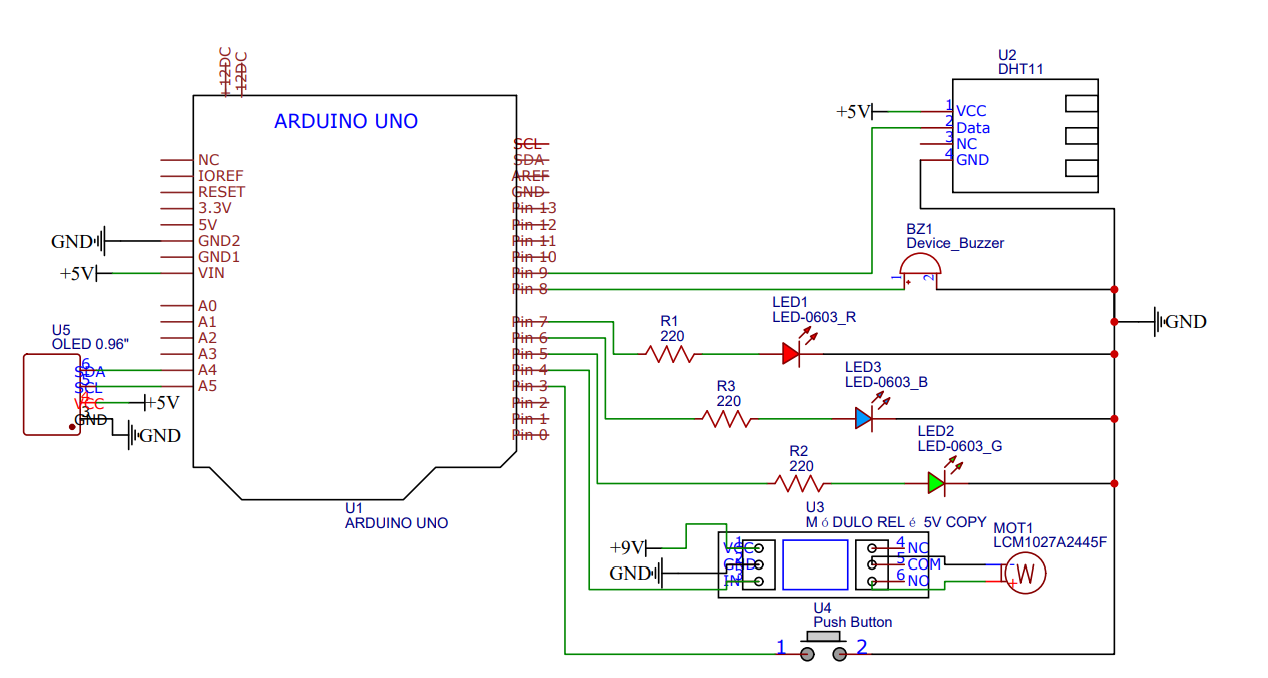
\includegraphics[width=\columnwidth]{images/Imagen_1R3.png}
                  \caption{Esquemático de Conexión Reto 3}
                  \label{fig:Imagen_1R3}
                  \end{figure}
                
            \end{itemize}
    
    \item Código Documentado

    El código propuesto documentado se encuentra registrado a continuación:
    \begin{lstlisting}[caption={Sistema de Riego Automatico con DHT11 y OLED}, label={lst:riego-automatico}]
#include <DHT.h>
#include <Adafruit_GFX.h>
#include <Adafruit_SSD1306.h>
// --- Definicion de pines ---
const int PIN_SENSOR_HUMEDAD = 2;
const int PIN_RELE           = 4;
const int PIN_LED_VERDE      = 5;
const int PIN_LED_AZUL       = 6;
const int PIN_LED_ROJO       = 7;
const int PIN_BUZZER         = 8;
const int PIN_BOTON_MANUAL   = 3;
// --- Configuracion DHT11 ---
#define DHTTYPE DHT11
DHT dht(PIN_SENSOR_HUMEDAD, DHTTYPE);
// --- Configuracion OLED ---
#define SCREEN_WIDTH 128
#define SCREEN_HEIGHT 64
#define OLED_RESET    -1
Adafruit_SSD1306 oled(SCREEN_WIDTH,
                      SCREEN_HEIGHT,
                      &Wire,
                      OLED_RESET);
// --- Umbrales de humedad ---
const int UMBRAL_SECO   = 30;
const int UMBRAL_HUMEDO = 70;
const int UMBRAL_ALARMA = 20;
const int HISTERESIS    = 5;
// --- Temporizacion ---
const long INTERVALO_LECTURA = 2000;
const long TIEMPO_MIN_RIEGO  = 5000;
// --- Enumeracion de estados ---
enum EstadoRiego
{ IDLE, REGANDO, ALARMA };
EstadoRiego estadoRiego = IDLE;
// --- Variables de control ---
float         humedadActual       = 0.0;
bool          bombaActiva         = false;
unsigned long tiempoUltimaLectura = 0;
unsigned long tiempoInicioRiego   = 0;
unsigned long tiempoBuzzer        = 0;
bool          estadoBuzzer        = false;
float leerHumedad() {
  float h = dht.readHumidity();
  if (isnan(h)) {
    Serial.println("Error DHT11");
    oled.clearDisplay();
    oled.setCursor(0, 0);
    oled.println("Error sensor");
    oled.println("DHT11 fallo");
    oled.display();
    return -1.0;
  }
  return h;
}
void activarBomba() {
  if (!bombaActiva) {
    digitalWrite(PIN_RELE, LOW);
    bombaActiva       = true;
    tiempoInicioRiego = millis();
    Serial.println("BOMBA: ACTIVADA");
  }
}
void desactivarBomba() {
  if (bombaActiva) {
    digitalWrite(PIN_RELE, HIGH);
    bombaActiva = false;
    Serial.println("BOMBA: DESACTIVADA");
  }
}
void evaluarEstadoRiego() {
  bool tiempoMinCumplido =
    (millis() - tiempoInicioRiego)
    >= TIEMPO_MIN_RIEGO;
  switch (estadoRiego) {
    case IDLE:
      if (humedadActual < UMBRAL_ALARMA){
        estadoRiego = ALARMA;
        activarBomba();
      } else if (humedadActual
                 <= UMBRAL_SECO) {
        estadoRiego = REGANDO;
        activarBomba();
      }
      break;
    case REGANDO:
      if (tiempoMinCumplido &&
          humedadActual >=
          UMBRAL_HUMEDO) {
        estadoRiego = IDLE;
        desactivarBomba();
      }
      break;
    case ALARMA:
      activarBomba();
      if (humedadActual >=
         (UMBRAL_SECO + HISTERESIS)) {
        estadoRiego = IDLE;
        desactivarBomba();
      }
      break;
  }
}
void actualizarIndicadores() {
  digitalWrite(PIN_LED_VERDE,
               estadoRiego == IDLE);
  digitalWrite(PIN_LED_AZUL,
               estadoRiego == REGANDO);
  digitalWrite(PIN_LED_ROJO,
               estadoRiego == ALARMA);
}
void gestionarBuzzerAlarma() {
  if (estadoRiego != ALARMA) {
    noTone(PIN_BUZZER);
    return;
  }
  if ((millis() - tiempoBuzzer) >= 500){
    tiempoBuzzer = millis();
    estadoBuzzer = !estadoBuzzer;
    if (estadoBuzzer)
      tone(PIN_BUZZER, 880, 250);
    else
      noTone(PIN_BUZZER);
  }
}
void verificarBotonManual() {
  if (digitalRead(PIN_BOTON_MANUAL)
      == LOW) {
    delay(50);
    if (digitalRead(PIN_BOTON_MANUAL)
        == LOW) {
      desactivarBomba();
      estadoRiego = IDLE;
      Serial.println(
        "OVERRIDE: Riego detenido");
    }
  }
}
void mostrarEnOLED() {
  oled.clearDisplay();
  oled.setTextSize(1);
  oled.setTextColor(SSD1306_WHITE);
  oled.setCursor(0, 0);
  oled.println("Sistema de Riego");
  oled.drawLine(0, 10, 127, 10,
                SSD1306_WHITE);
  oled.setTextSize(2);
  oled.setCursor(0, 16);
  oled.print("Hum: ");
  oled.print((int)humedadActual);
  oled.println("%");
  oled.setTextSize(1);
  oled.setCursor(0, 40);
  oled.print("Estado: ");
  switch (estadoRiego) {
    case IDLE:
      oled.println("OPTIMO");   break;
    case REGANDO:
      oled.println("REGANDO");  break;
    case ALARMA:
      oled.println("ALARMA!");  break;
  }
  oled.setCursor(0, 52);
  oled.print("Bomba: ");
  oled.println(bombaActiva ?
  "ON":"OFF");
  oled.display();
}
void setup() {
  Serial.begin(9600);
  dht.begin();
  pinMode(PIN_RELE,         OUTPUT);
  pinMode(PIN_LED_VERDE,    OUTPUT);
  pinMode(PIN_LED_AZUL,     OUTPUT);
  pinMode(PIN_LED_ROJO,     OUTPUT);
  pinMode(PIN_BUZZER,       OUTPUT);
  pinMode(PIN_BOTON_MANUAL,
  INPUT_PULLUP);
  digitalWrite(PIN_RELE, HIGH);
  oled.begin(SSD1306_SWITCHCAPVCC,
             0x3C);
  oled.clearDisplay();
  oled.setTextSize(1);
  oled.setTextColor(SSD1306_WHITE);
  oled.setCursor(20, 20);
  oled.println("Sistema Riego");
  oled.setCursor(25, 35);
  oled.println("Iniciando...");
  oled.display();
  delay(2000);
  oled.clearDisplay();
  Serial.println(
    "Sistema de Riego - Listo");
}
void loop() {
  unsigned long ahora = millis();
  if (ahora - tiempoUltimaLectura
      >= INTERVALO_LECTURA) {
    tiempoUltimaLectura = ahora;
    humedadActual = leerHumedad();
    if (humedadActual < 0) return;
    evaluarEstadoRiego();
    actualizarIndicadores();
    mostrarEnOLED();
    Serial.print("Humedad: ");
    Serial.print(humedadActual);
    Serial.print("% | Estado: ");
    Serial.println(estadoRiego);
  }
  gestionarBuzzerAlarma();
  verificarBotonManual();
}
\end{lstlisting}
\end{itemize}
        










\section{Protocolos de Comunicación}\label{sec:protocolosdecomunicacion}
  \begin{itemize}
    \item ¿Por qué no basta con "tener Wi-Fi"?
    Una solución IoT completa involucra múltiples capas de comunicación. Algunas se encargan de conectar sensores al microcontrolador, otras permiten enlazar el nodo con internet, y otras definen cómo se intercambian los datos a nivel de aplicación. Reducir el IoT únicamente a la conectividad Wi-Fi constituye un error conceptual frecuente, ya que ignora la complejidad real de los sistemas embebidos conectados.

    \begin{itemize}
        \item Comunicación interna del nodo embebido (dentro del hardware)
        Antes de transmitir información a la red, el sistema debe capturar y procesar correctamente los datos provenientes de los sensores:

        \begin{itemize}
            \item GPIO y señales digitales: lectura de estados y activación de actuadores.
            \item Entradas analógicas y ADC: adquisición de variables continuas como temperatura o presión.
            \item PWM: control de velocidad, intensidad luminosa o posición.
            \item I2C: comunicación con múltiples sensores usando pocos conductores.
            \item SPI: transmisión de alta velocidad con memorias, pantallas o sensores especializados.
            \item UART: comunicación serial para depuración o conexión con módulos externos.
        \end{itemize}

        \item Tecnologías inalámbricas para conectar el nodo a la red

        La selección de la tecnología de comunicación depende del equilibrio entre alcance, consumo energético, velocidad de transmisión y costo de implementación. En la Tabla~\ref{tab:Tabla_4_PDCIoT} se resumen las tecnologías más utilizadas.

        \begin{table*}
    

\centering
\renewcommand{\arraystretch}{1.3}
\label{tab:Tabla_4_PDCIoT}
\begin{tabular}{|l|c|c|c|p{2cm}|}
\hline
\textbf{Tecnología} & \textbf{Alcance} & \textbf{Consumo} & \textbf{Tasa de datos} & \textbf{Uso típico} \\
\hline
Wi-Fi & $\sim$100 m & Alto & Hasta 1 Gbps & Hogares, oficinas, prototipos ESP32 \\
\hline
Bluetooth / BLE & 10--100 m & Bajo & 1--3 Mbps & Wearables, sensores cercanos \\
\hline
ZigBee & $\sim$100 m & Bajo & 250 kbps & Domótica, automatización industrial \\
\hline
LoRa / LPWAN & 2--15 km & Muy bajo & 0.3--50 kbps & Agricultura, ciudades inteligentes, campo abierto \\
\hline
NFC / RFID & $<$ 10 cm & Muy bajo & 424 kbps & Identificación, pagos, logística \\
\hline
Celular 4G/5G & Km & Variable & Hasta Gbps & Vehículos, monitoreo remoto sin red local \\
\hline
Ethernet & Cableado & Bajo/medio & Alta & Ambientes industriales fijos, alta estabilidad \\
\hline
\end{tabular}
\caption{Tecnologías inalámbricas para conectar el nodo a la red}
\label{tab:tecnologias_inalambricas}
\end{table*}[h]

        No existe una tecnología universalmente superior; la elección depende del caso de uso específico.

        \item Notas específicas de cada tecnología

        \begin{itemize}
            \item Wi-Fi: basado en el estándar 802.11, ideal para transmisión de grandes volúmenes de datos y conexión directa a internet.
            \item Bluetooth / BLE: optimizado para bajo consumo, fundamental en dispositivos portátiles y sensores de batería.
            \item ZigBee: diseñado para redes de sensores distribuidos que operan de forma cooperativa.
            \item Thread: protocolo mallado basado en IPv6, auto-reparable y eficiente energéticamente.
            \item LoRaWAN: orientado a telemetría de largo alcance con bajo consumo y baja frecuencia de transmisión.
            \item Celular / NB-IoT: permite independencia de redes locales, aunque con mayor complejidad operativa.
        \end{itemize}

        \item Protocolos de aplicación: cómo se empaqueta y transporta la información

        Una vez establecida la conexión de red, es necesario definir el protocolo de intercambio de datos:

        \begin{itemize}
            \item HTTP / REST: modelo cliente-servidor basado en solicitudes y respuestas. Adecuado para servicios web y pruebas iniciales.
            \item MQTT: protocolo ligero basado en publicador/suscriptor, altamente eficiente para telemetría y sistemas distribuidos. El broker gestiona la distribución de mensajes.
            \item WebSocket: permite comunicación bidireccional continua mediante conexión persistente, útil para dashboards y control en tiempo real.
        \end{itemize}

        En aplicaciones con ESP32, MQTT resulta especialmente formativo para comprender la lógica IoT, mientras que HTTP facilita la integración con servicios web.

        \item Criterio de selección resumido

        No existe una solución única óptima. La elección adecuada surge del análisis de los requerimientos del sistema:

        \begin{itemize}
            \item ¿Qué alcance de comunicación se necesita?
            \item ¿Qué volumen de datos se transmitirá y con qué frecuencia?
            \item ¿Cuál es el consumo energético permitido?
            \item ¿Cuál es el costo y la facilidad de implementación en el entorno específico?
        \end{itemize}

    \end{itemize}
\end{itemize}

\section{IoT VS Internet Convencional}\label{sec:iotvsinternet}
  \begin{itemize}

    \item ¿Qué es el IoT y de dónde viene?

    El término ``Internet de las Cosas'' fue acuñado por Kevin Ashton en 1999, en el contexto del MIT, para describir la idea de conectar objetos físicos a internet mediante etiquetas RFID. Su consolidación como paradigma tecnológico dependió del avance simultáneo de tres factores: el desarrollo de microcontroladores cada vez más pequeños, económicos y eficientes; la masificación de la conectividad inalámbrica; y la adopción del protocolo IPv6, que permitió asignar direcciones únicas a miles de millones de dispositivos. El cambio fundamental no fue solo conectar dispositivos, sino convertir el entorno físico en una fuente permanente de datos útiles para supervisión, decisión y acción.

        \begin{itemize}

            \item Diferencia conceptual entre los tres paradigmas

            En el \textbf{internet tradicional}, la interacción ocurre entre personas y servicios web: el usuario consulta, descarga o accede a plataformas. Los datos son texto, imagen, audio o video, y el flujo es persona $\rightarrow$ red $\rightarrow$ servicio. La generación de datos depende completamente de la acción deliberada del usuario humano; sin interacción, no hay dato.

            En el \textbf{IoT}, los objetos físicos captan, procesan y comunican datos de forma autónoma. El entorno físico se convierte en fuente permanente de información sin requerir intervención humana directa. El flujo cambia a: sensor $\rightarrow$ procesamiento $\rightarrow$ red $\rightarrow$ decisión $\rightarrow$ acción. Los datos dominantes son variables físicas del entorno como temperatura, humedad, presión o posición. Los objetivos son el monitoreo, control y automatización distribuida. Ejemplos representativos incluyen estaciones ambientales, casas inteligentes y sistemas de riego automatizado.

            En el \textbf{IIoT} (Internet Industrial de las Cosas), los nodos se integran con máquinas, procesos industriales, líneas de producción, inventarios y sistemas de trazabilidad. Los datos dominantes son variables de proceso, estado de activos, calidad y trazabilidad productiva. El objetivo central es la optimización operativa, el mantenimiento predictivo, la eficiencia energética y la producción inteligente. A diferencia del IoT doméstico o académico, el IIoT opera bajo requisitos más estrictos de confiabilidad, latencia y seguridad.

            En la \textbf{Industria 4.0}, el dato deja de ser solo un registro histórico y se convierte en base para analítica avanzada, interoperabilidad entre sistemas heterogéneos, decisión en tiempo real y automatización inteligente apoyada en inteligencia artificial y gemelos digitales.

            \item IoT desde la perspectiva de sistemas embebidos

            Un sistema embebido en el contexto IoT deja de ser un dispositivo aislado y se convierte en un nodo activo dentro de una arquitectura mayor. Para cumplir este rol, debe integrar cinco funciones fundamentales:

                \begin{itemize}
                    \item \textbf{Sensar:} captar variables físicas del entorno mediante sensores de temperatura, humedad, presión, corriente, vibración, posición, entre otros.
                    \item \textbf{Procesar:} acondicionar, filtrar, escalar, convertir y organizar los datos dentro del microcontrolador o en una etapa de procesamiento en el borde (\textit{edge computing}).
                    \item \textbf{Comunicar:} transmitir la información hacia otros nodos o hacia internet mediante un medio físico y un protocolo de aplicación apropiados al contexto.
                    \item \textbf{Visualizar o almacenar:} presentar los datos al usuario final a través de dashboards o interfaces web, o registrarlos en bases de datos para análisis posterior.
                    \item \textbf{Actuar:} ejecutar decisiones que modifiquen el proceso físico mediante relés, válvulas, motores, alarmas o consignas de control.
                \end{itemize}

            La idea clave es que el microcontrolador no es el sistema completo, sino únicamente el nodo local. El valor real del IoT aparece cuando el dato sale del dispositivo, viaja por la red, se integra con información de otros nodos y se convierte en conocimiento útil para tomar decisiones concretas.

            \item Arquitectura por capas de un sistema IoT

            Los sistemas IoT se organizan típicamente en una arquitectura de cuatro capas, cada una con una función específica dentro del flujo del dato:

                \begin{itemize}
                    \item \textbf{Capa física o de percepción:} contiene los sensores, actuadores, el microcontrolador, conversores ADC y pines GPIO. Es el punto de contacto directo con el mundo físico. Pregunta de diseño: ¿qué se mide, con qué precisión, con qué frecuencia de muestreo y qué variables se controlan?
                    \item \textbf{Capa de comunicación:} se encarga de mover la información desde la capa física hacia internet o hacia otros nodos. Incluye tecnologías como Wi-Fi, BLE, Zigbee, LoRa, Ethernet, redes móviles y gateways intermediarios. Pregunta de diseño: ¿qué alcance se necesita, qué consumo energético es aceptable, qué protocolo conviene según el volumen y frecuencia de datos?
                    \item \textbf{Capa de servicio:} gestiona la recepción, almacenamiento, procesamiento y protección de los datos. Incluye brokers MQTT, bases de datos relacionales o de series temporales, servidores web, APIs REST, dashboards de visualización, reglas de negocio y sistemas de alertas. Pregunta de diseño: ¿dónde se almacenan los datos, cómo se visualizan en tiempo real, qué nivel de seguridad y autenticación se requiere?
                    \item \textbf{Capa de aplicación:} es la que entrega valor directo al usuario o al proceso. Habilita funciones de monitoreo remoto, control automatizado, predicción de fallos, mantenimiento preventivo, trazabilidad de activos y optimización logística. Pregunta de diseño: ¿qué decisión concreta permite tomar el sistema, qué indicador operativo mejora?
                \end{itemize}

            \item Transición IoT $\rightarrow$ IIoT $\rightarrow$ Industria 4.0 en síntesis

                \begin{itemize}
                    \item \textbf{IoT:} monitorea variables ambientales o de dispositivos individuales en contextos domésticos, urbanos o académicos. El alcance es limitado y los requisitos de confiabilidad son moderados.
                    \item \textbf{IIoT:} integra datos de múltiples nodos distribuidos para mejorar productividad, disponibilidad de activos, seguridad operacional y calidad del producto en entornos industriales exigentes.
                    \item \textbf{Industria 4.0:} el dato se convierte en el recurso central. Se habilitan capacidades de analítica avanzada, interoperabilidad entre sistemas heterogéneos, automatización inteligente y decisión en tiempo real apoyada en modelos predictivos.
                \end{itemize}

            \item Desafíos recurrentes que no deben ignorarse

            Independientemente de la escala del sistema IoT, existen desafíos transversales que deben considerarse desde las etapas iniciales del diseño:

                \begin{itemize}
                    \item \textbf{Seguridad:} proteger credenciales de acceso, cifrar los canales de comunicación y controlar el acceso a los datos almacenados. Un sistema IoT mal asegurado representa un vector de ataque crítico.
                    \item \textbf{Energía:} estimar el consumo de cada componente, definir la autonomía requerida y seleccionar el tipo de alimentación adecuado, especialmente en nodos remotos alimentados por batería o energía solar.
                    \item \textbf{Robustez:} prever y gestionar situaciones de pérdida de conexión, reinicios inesperados, errores de lectura de sensores y condiciones ambientales adversas. El sistema debe recuperarse de forma autónoma.
                    \item \textbf{Escalabilidad:} diseñar la arquitectura de modo que funcione correctamente con un nodo, con diez o con una red de cientos de dispositivos, sin requerir rediseños estructurales.
                    \item \textbf{Mantenibilidad:} documentar con claridad las conexiones físicas, las variables del sistema, los formatos de mensaje, las versiones de librerías y las dependencias de software, para facilitar el mantenimiento y la actualización futura del sistema.
                \end{itemize}

        \end{itemize}

\end{itemize}

\section{Resultados y discusión}\label{sec:resultados}
  % Resultados: presenta tablas/figuras y comenta hallazgos clave.

%\subsection{Ejemplo de figura} % Sub-sección para ilustrar resultados gráficos
% \begin{figure}[!t]             % Entorno de figura; [!t]=arriba, con preferencia fuerte (!)
 %  \centering
  % includegraphics: inserta imagen externa
  % keepaspectratio: conserva la relación de aspecto al escalar
  % width=0.9\linewidth: ancho al 90% de la línea actual (se puede usar height=...)
%   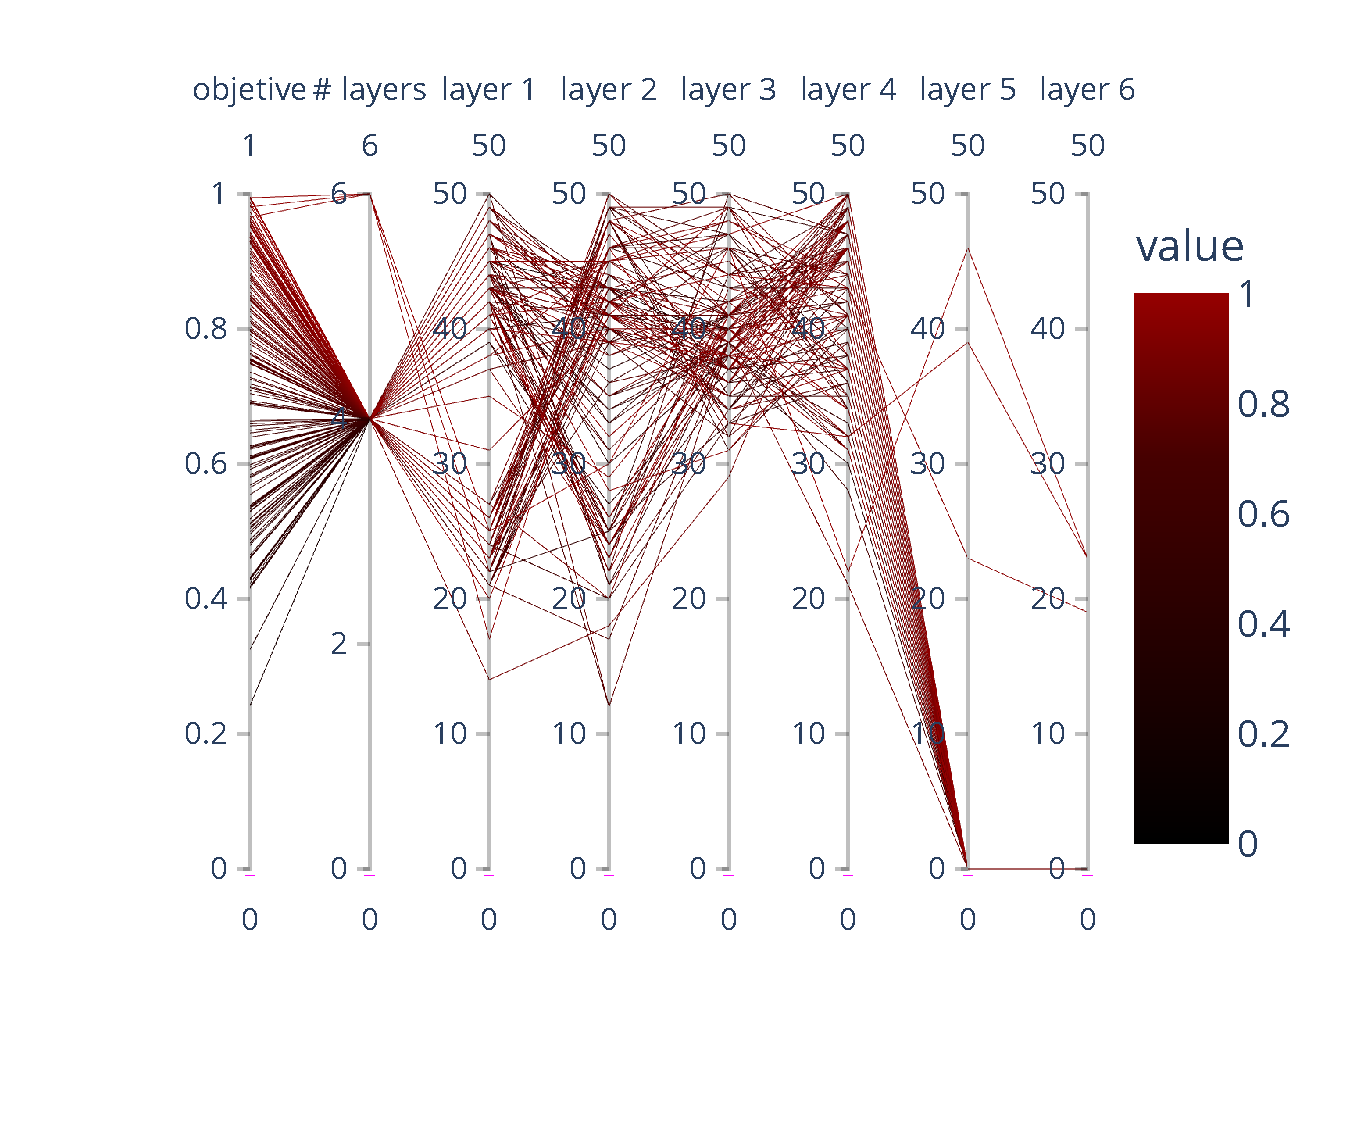
\includegraphics[keepaspectratio, width=0.9\linewidth]{images/neurons.pdf}
%   \caption{Figura de ejemplo generada con PGF (sustituible por tus resultados).} % Texto bajo la figura
%   \label{fig:res_fig}          % Etiqueta para referenciar con \ref{fig:res_fig}
% \end{figure}

%\subsection{Ejemplo de tabla}  % Sub-sección para resultados en formato tabla
 % \input{tables/table2.tex}      % Inserta archivo de tabla externa en este punto

% Consejos: Compara contra una línea base y reporta métricas con su interpretación.

\section{Conclusiones}\label{sec:conclusiones}
  % Conclusiones: 3–5 viñetas claras. Incluye trabajo futuro.

En esta plantilla:

- Se mostró la estructura básica de un artículo IEEEtran en LaTeX en español.
- Se incluyeron ejemplos mínimos de figuras, tablas, ecuaciones y citas.
- Se proporcionaron comentarios en el código para guiar el uso en clase.

Trabajo futuro: reemplazar el contenido de ejemplo por el de tu proyecto, añadir más secciones si es necesario y ajustar el preámbulo según las normas de la conferencia o revista.

% La sección de agradecimientos es opcional y no está numerada.
\section*{Agradecimientos}\label{sec:agradecimientos}
  % Agradecimientos
Los autores agradecen a la Dra.\ Edna Carolina Moriones Polanía, docente del curso de Sistemas Embebidos de la Universidad Santo Tomás – Seccional Bucaramanga, por el planteamiento del proyecto, la definición de los requisitos técnicos a través del Acta de Solicitudes del Cliente, y el acompañamiento durante el desarrollo del semestre. Así mismo, se agradece a la institución por facilitar el acceso al laboratorio y los materiales de prototipado necesarios para la implementación del sistema.


% ===================================================================
% BIBLIOGRAFÍA
% ===================================================================
% Define el estilo de la bibliografía (IEEEtran es el estándar).
% Añade tus referencias en el archivo 'reference.bib'.
\bibliographystyle{IEEEtran}


\footnotesize\bibliography{reference}

\end{document}
